\section{Objetivo del capítulo}

En este capítulo se presenta una familia de implementaciones de \setchain de mundo
real construidas sobre Tendermint.
%
En particular, se exponen tres alternativas diferentes, comenzando con una
solución simple pero trivialmente correcta y finalizando con un algoritmo
complejo que implementa \setchain utilizando funciones hash.
%

\section{Consideraciones generales}\label{sec:impl}
Para evitar repeticiones, algunas definciones de métodos que permanezcan sin cambios
de una versión a la siguiente, no serán re-escritas.
Esto será debidamente aclarado al momento de la presentación de los algoritmos.

%
A su vez, con la intención de mantener consistencia en la nomenclatura,
el término \textit{transacción} se utiliza siempre para referirse a las
\textit{transacciones de Tendermint}, mientras
que \textit{elemento} queda reservado para elementos a agregarse a la \setchain.
%
Dependiendo de la alternativa sobre la que se esté trabajando, una transacción de
Tendermint puede contener uno o más elementos a ser agregados.
%
% \subsection{General Considerations about Implementation}\label{subsec:general}

Las implementaciones correctas de \setchain implementan dos métodos~(ver sección
~\ref{sec:setchain}): \<add> y \<get>, por lo tanto, cada solución provee definiciones
para ambas.
%
Por su parte, Tendermint provee dos \textit{endpoints} RPC principales.
Nótese que el cliente siempre se comunica con un nodo particular de la red de servidores.
\begin{itemize}
  \item \texttt{Tendermint.Broadcast} se utiliza para enviar transacciones.
  Cuando una transacción es enviada, se chequea si dicha transacción
  es válida contra la aplicación (mediante la llamada a \<CheckTx>), y en caso
  afirmativo, se añade
  a la mempool, se difunde a los otros nodos y eventualmente se incluye en
  un bloque.
  \item \<abciquery> se utiliza para consultar el estado de la
  aplicación.
\end{itemize}
%

% Important: Note the mempool does not provide strong guarantees - just because a tx
% passed CheckTx (ie. was accepted into the mempool), doesn't mean it will be committed,
% as nodes with the tx in their mempool may crash before they get to propose.

Por lo tanto, desde el punto de vista del cliente de la \setchain, solo existen dos
métodos (\<add> y \<get>).
%
Sin embargo, hay dos métodos adicionales que se utilizan internamente (es decir, desde
el punto de vista de la programadora) para comunicarse
con la red de Tendermint subyacente (los ya mencionados \texttt{Tendermint.Broadcast} y
\texttt{Tendermint.Query}).
%

Finalmente, se asume que hay un predicado definido por el usuario que define
cuándo un elemento es válido para ser admitido en el conjunto.
%
En esta sección, dicho predicado se referencia con la función \<isValidElement>.
%
De este modo, llamaremos \textit{elementos válidos} a aquellos elementos $e$ para los cuales
$\<isValidElement>(e)$ retorne verdadero.

%
A continuación se presentan diferentes definiciones de métodos
necesarios para que la aplicación corriendo sobre Tendermint implemente \setchain.
Esto involucra, por un lado, los métodos presentados como parte de la API de
\setchain y, por el otro, los perteniences a la interfaz de aplicación de
blockchain ~(ver sección ~\ref{sec:tendermint}). Si bien el objetivo del capítulo es
presentar las soluciones a nivel conceptual, detalles de implementación son dados a lo largo
de las secciones cuando se considera oportuno.

\section{Primera implementación: \vanilla}\label{sec:vanilla}

\vanilla se presenta como la solución más sencilla a la API de \setchain
utilizando Tendermint.
%
La característica principal que le otorga sencillez a esta solución es que
un cliente invocando $v.$\<add>(e) sobre un servidor correcto $v$ se
traduce en una nueva transacción de Tendermint en la red,
que representa a ese y solo a ese elemento a añadir a la \setchain.
%
Que $e$ sea finalmente añadido a la \setchain dependerá de si la transacción asociada
al mismo se incluye en un bloque que, a su vez, eventualmente se agrega a la blockchain
subyacente de Tendermint.

Otro aspecto fundamental de esta solución es que cada bloque de Tendermint
define una única época de \setchain, a la cual pertenecen todos los elementos asociados
a las transacciones en dicho bloque.

\subsection{Flujo de mensajes}

\begin{figure}
  \subfloat[Estado inicial]{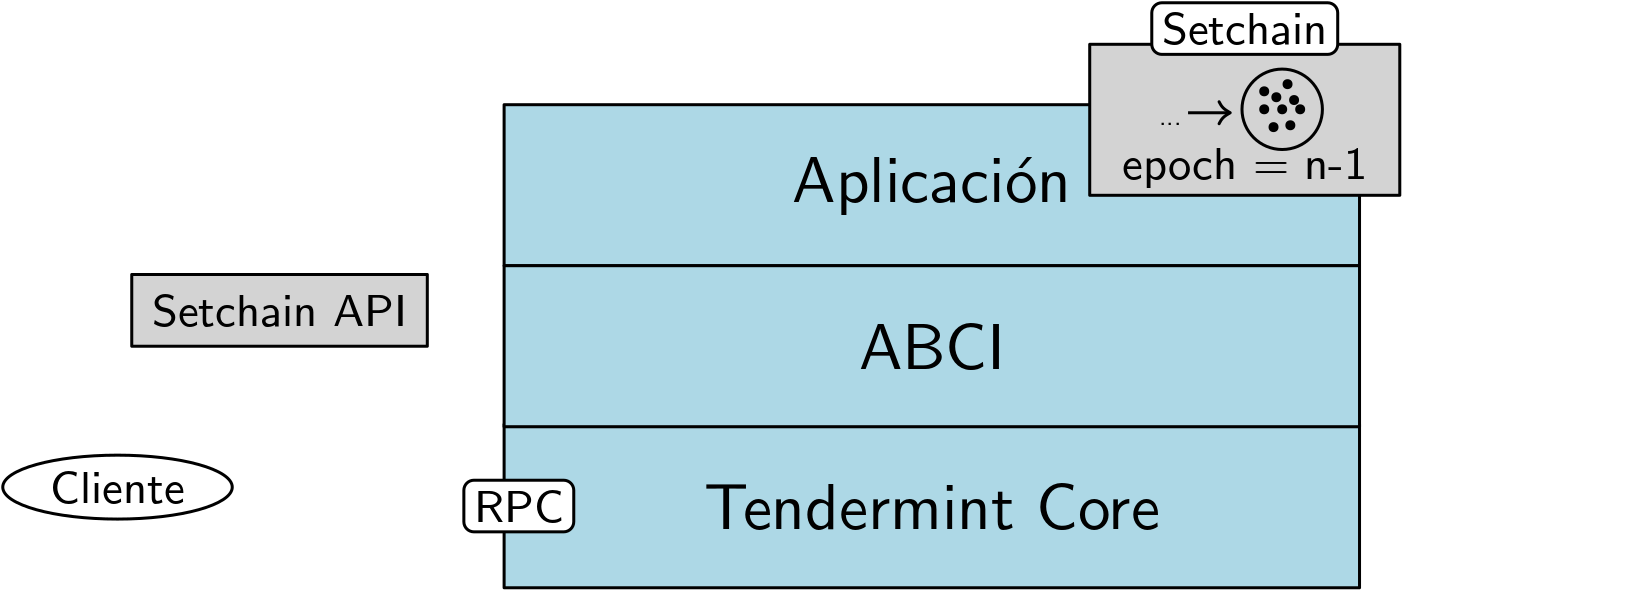
\includegraphics[width = 3in]{figures/vanilla-reflow-0.png}\label{subfig:vanilla-flow-a}}
  \subfloat[El cliente invoca \<add>(e)]{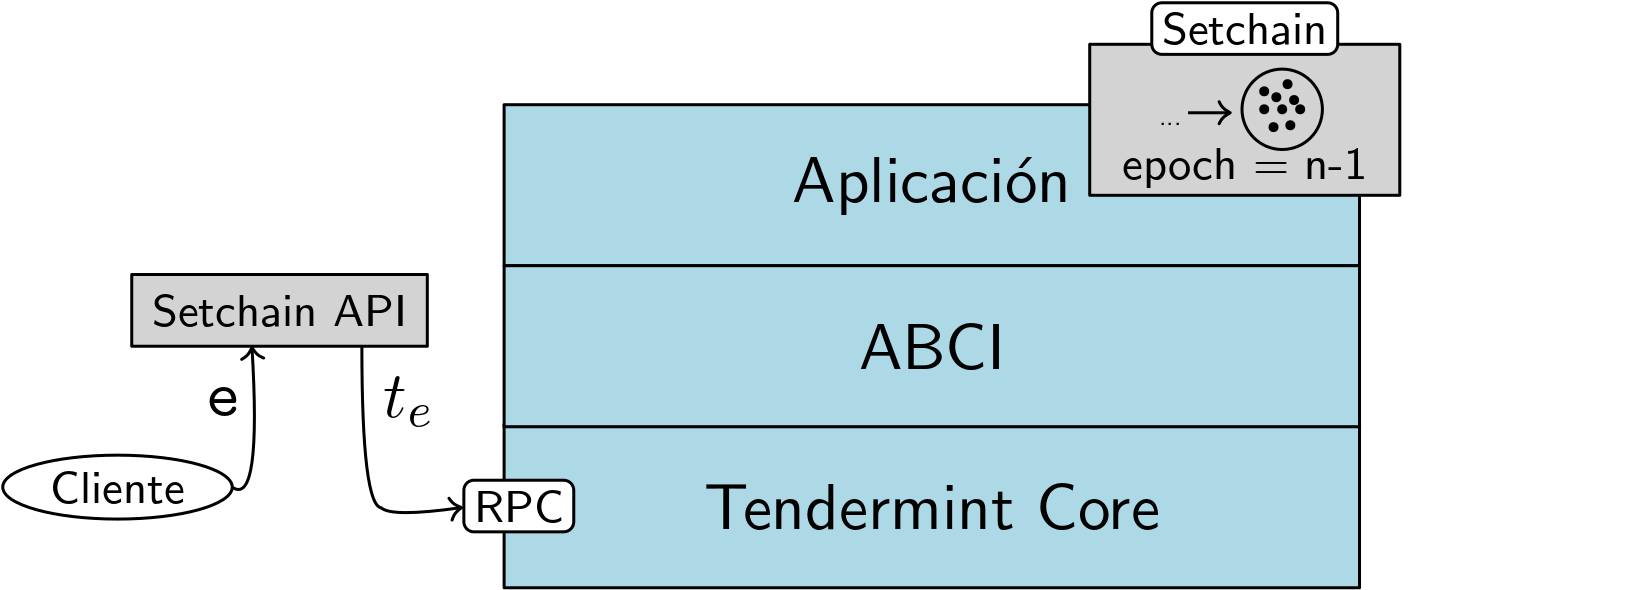
\includegraphics[width = 3in]{figures/vanilla-reflow-1.png}\label{subfig:vanilla-flow-b}}\\
  \vspace{0.5cm}
  \subfloat[$t_e$ se chequea contra \CheckTx]{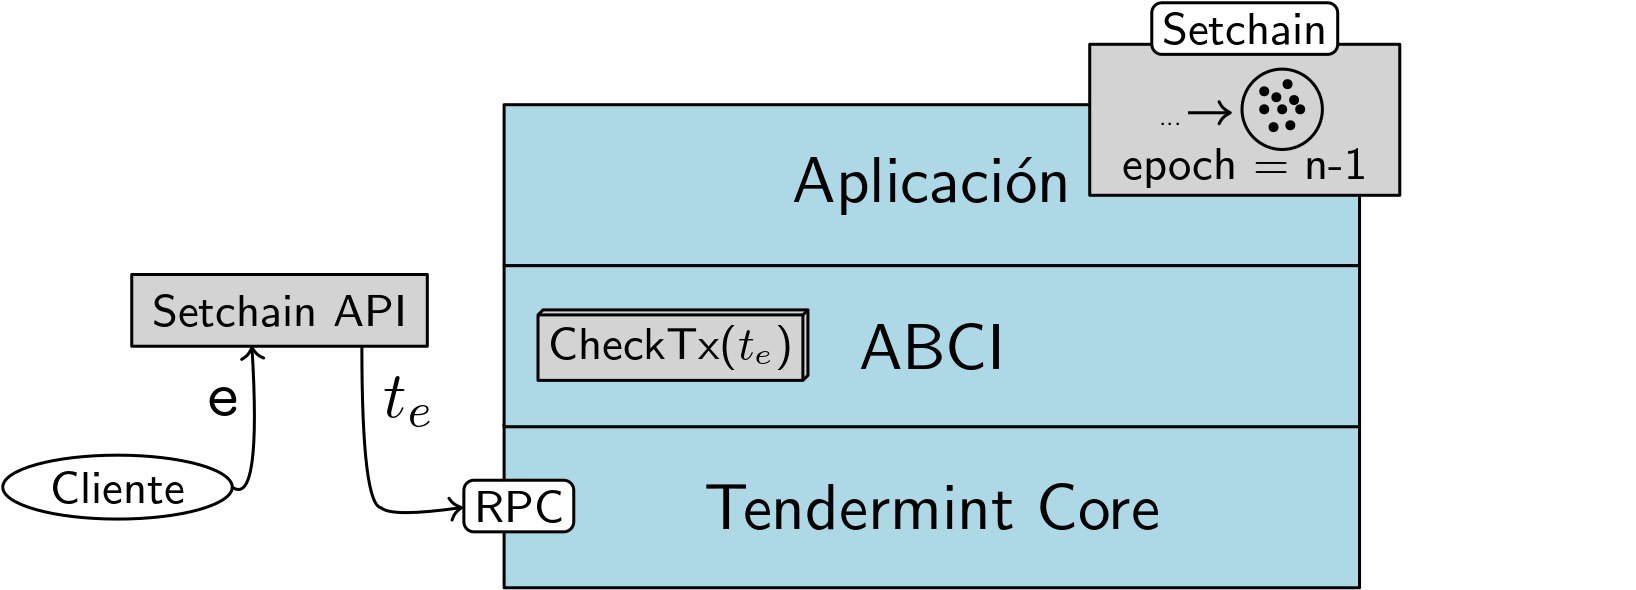
\includegraphics[width = 3in]{figures/vanilla-reflow-2.png}\label{subfig:vanilla-flow-c}}
  \subfloat[Se consensúa el próximo bloque]{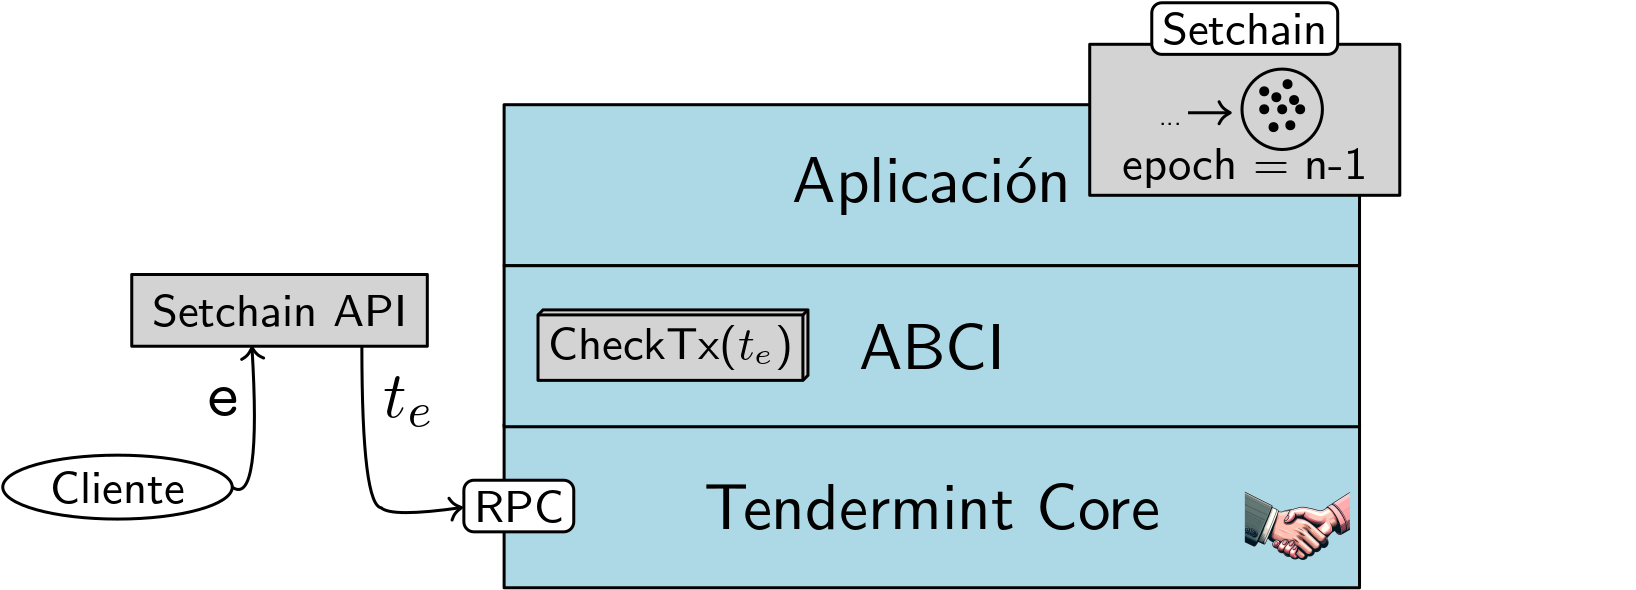
\includegraphics[width = 3in]{figures/vanilla-reflow-3.png}\label{subfig:vanilla-flow-d}}\\
  \vspace{0.5cm}
  \subfloat[Se envían los pedidos de la ABCI a la aplicación]{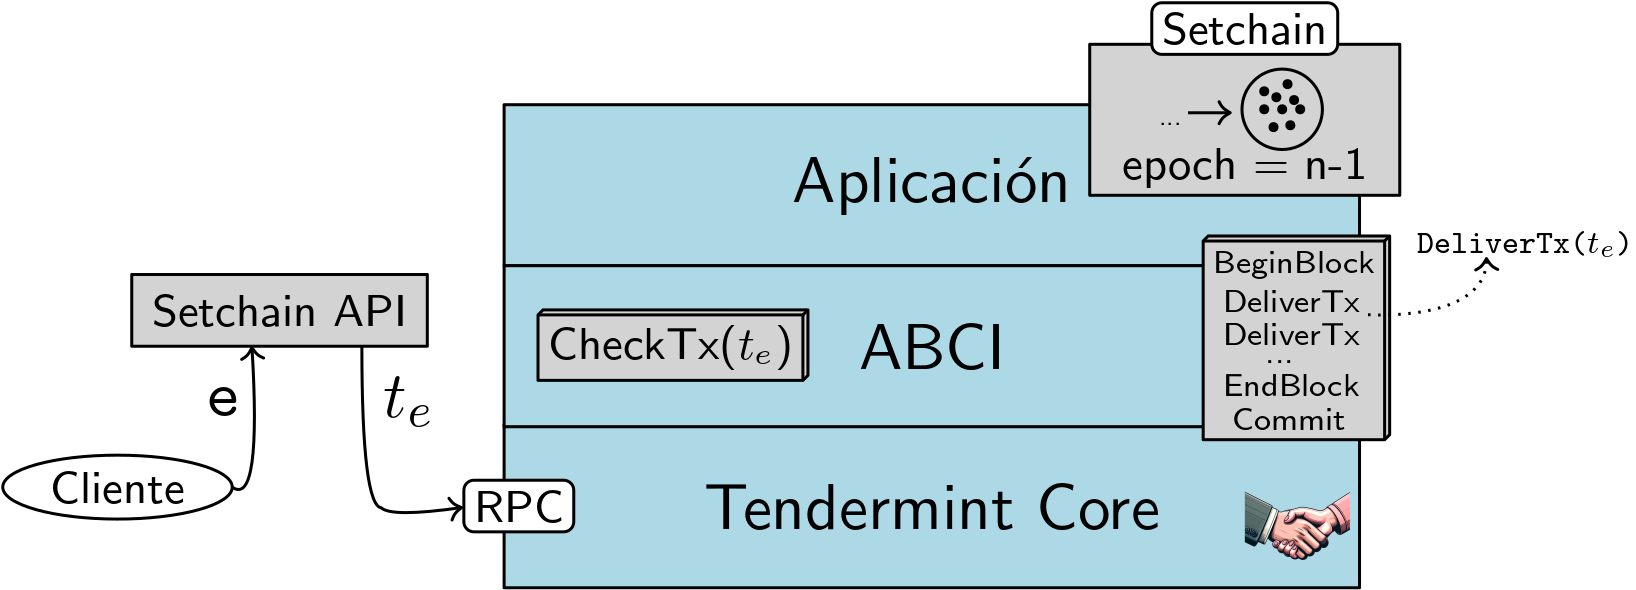
\includegraphics[width = 3in]{figures/vanilla-reflow-4.png}\label{subfig:vanilla-flow-e}}
  \subfloat[Se agrega la época $n$ a la \setchain]{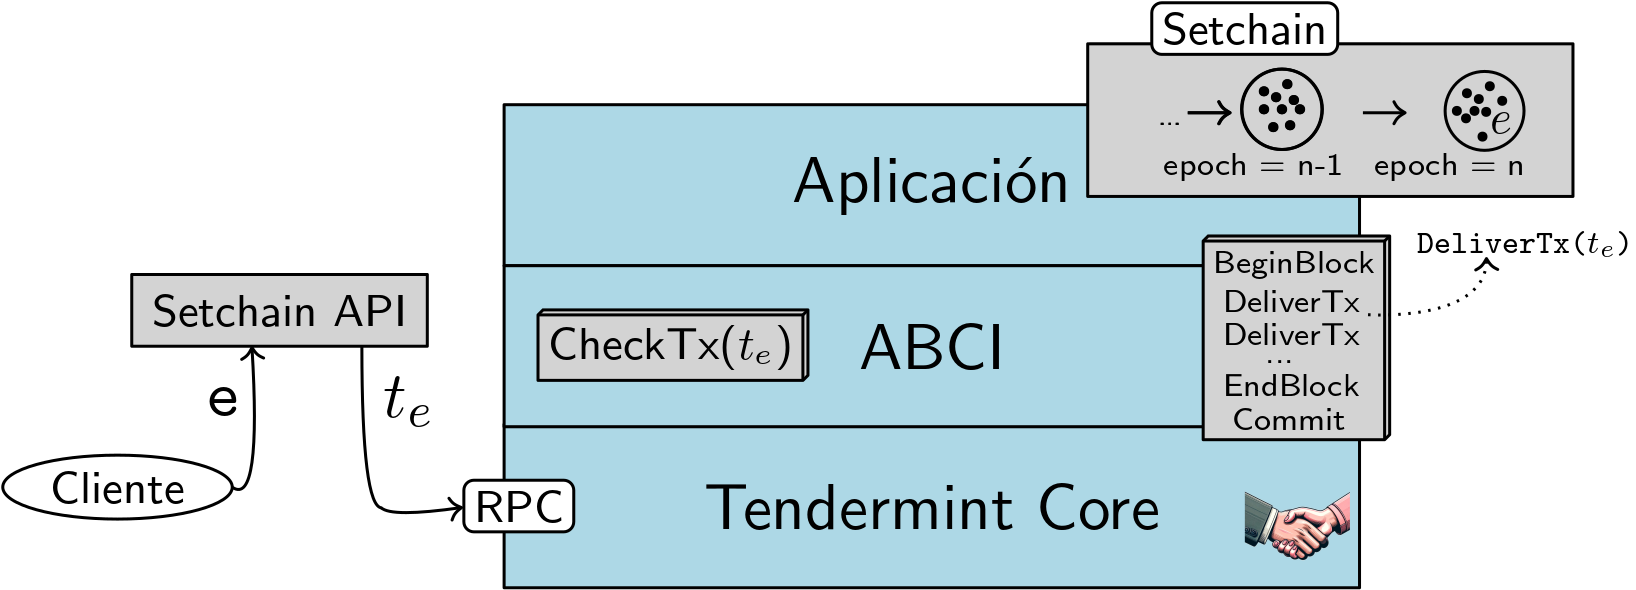
\includegraphics[width = 3in]{figures/vanilla-reflow-5.png}\label{subfig:vanilla-flow-f}}
  \caption{Flujo usual de mensajes para \vanilla}
  \label{fig:vanilla-flow}
\end{figure}

En la Figura~\ref{fig:vanilla-flow} se muestra el flujo usual de mensajes que se inicia
cuando un cliente invoca $v.$\<add>(e) sobre un servidor correcto $v$.
%

El sistema comienza en su estado inicial (Figura \ref{subfig:vanilla-flow-a}), a la espera de que algún cliente
se conecte con ese nodo (parte de la red) para agregar un elemento.
El Tendermint Core expone sus puntos de entrada RPC, que serán utilizados por parte de la API de
\setchain. Por su parte, la aplicación es quien se encargará de acceder a la base de datos persistente que
mantiene la estructura distribuida que conforma la \setchain.
%

En la Figura \ref{subfig:vanilla-flow-b} se observa el resultado de un cliente invocando \<add>(e): el cliente, mediante
la API de \setchain, envía un elemento $e$, y la API de \setchain, a su vez, se comunica con el
punto de entrada del Tendermint Core para enviar una transacción $t_e$ que representa a $e$.
Si bien el cliente envía \textit{elementos}, en la red de Tendermint
lo que circulan son \textit{transacciones}.
%

Para determinar si la nueva transacción debe ser difundida en la red, Tendermint chequea que
sea válida por medio de \CheckTx, y si lo es, entonces inserta la transacción en la mempool.
En caso contrario, la descartará, el flujo de dicha transacción terminará y el elemento $e$
asociado a ella no será agregado a la \setchain.
La petición \CheckTx se muestra en la Figura \ref{subfig:vanilla-flow-c}.

%
Si la transacción $t_e$ llega a la mempool, luego de un tiempo, es esperable que sea añadida a un
bloque de Tendermint, propuesto como siguiente bloque en la cadena, como parte del algoritmo de
consenso.
Una vez que dicho bloque obtiene todos los votos necesarios para ser considerado
\textit{commited by the network}, comenzará una nueva instancia de consenso. En la Figura \ref{subfig:vanilla-flow-d}
se representa que el siguiente bloque fue consensuado por parte del Tendermint Core.

%
El siguiente paso será que el Tendermint Core envíe
la secuencia correspondiente de pedidos a la aplicación: \BeginBlock para indicar el inicio de
un nuevo bloque,
una lista de llamadas a \DeliverTx por cada transacción agregada\footnote{En esta implementación
una \textit{transacción} agregada coincide con un \textit{elemento} agregado.} (en el orden en que fueron
consensuadas dentro del bloque),
\EndBlock para indicar la finalización del bloque y \Commit para señalizar que el nuevo estado
puede ser persistido.
%
Si la transacción $t_e$ de Tendermint asociada a $e$ es parte de dicho bloque,
entonces con seguridad, una de las llamadas a \DeliverTx tendrá como argumento a $t_e$.
Esto se visualiza en la Figura \ref{subfig:vanilla-flow-e}.

%
El último paso en este flujo (Figura \ref{subfig:vanilla-flow-f}) muestra que una nueva época se agregó a la \setchain,
en donde uno de sus elementos es $e$.

\subsubsection{Detalles de implementación}
La implementación de la API de \setchain establece comunicación con un nodo mediante el protocolo HTTP.
%
Se utiliza la implementación nativa de Tendermint del cliente HTTP,
quien se comunica con el nodo de Tendermint usando JSON RPC.
%
De los distintos clientes nativos que provee Tendermint, el cliente HTTP
es la implementación más adecuada de utilizar en un entorno
real, y es por eso que se elige para este trabajo.

La aplicación necesita acceso a una base de datos persistente, de modo de ir añadiendo
los elementos correspondientes a cada época de la \setchain.
%
Esta base de datos persistente se implementa utilizando el paquete \textit{BadgerDB}\cite{db.badger},
que provee una base de datos simple y rápida de tipo clave-valor, escrita completamente en Go.
%
Dependiendo del caso de uso de \setchain se pueden pensar distintas formas de almacenar los elementos y sus
respectivas épocas, de modo de hacer más eficiente las búsquedas necesarias.
%
Por ejemplo, si fuera importante determinar rápidamente si un elemento ya es parte de la \setchain y con cuál número de época
fue estampado, entonces, al agregar un nueva entrada a la base de datos, las claves podrían ser elementos, y los
valores, el número de época al que dicho elemento pertenece.
%
Por otro lado, si se quisiera dar mayor eficiencia a determinar todos los elementos pertenecientes a una época dada,
los valores podrían ser números de épocas, y las claves los elementos en ella.
%
Incluso podría utilizarse un sistema híbrido, de modo de hacer eficiente diversas búsquedas.

\subsection{Prueba de membrecía de elementos}\label{subsubsec:membership}
%
Como se mencionó antes, cuando un proceso cliente utiliza la API de \setchain
para añadir un elemento o para recuperar el estado actual de la \setchain,
se comunica con un nodo particular de la red. Es importante notar que, en este
sentido, un proceso cliente no puede saber si se está contactando con un nodo
correcto o con un nodo bizantino.
%Client processes do not know if they are contacting a Byzantine or correct
%process.
%
Para asegurar que un elemento será añadido a la \setchain, el cliente necesitaría
interactuar con suficientes servidores, de modo de garantizar que al menos uno de ellos
sea correcto.
%
% An extension to Setchain presented an optimistic client with the following
% approach.
%
Como ya se mencionó en el modelo de computación (ver Sección ~\ref{sec:model_system}),
se asume que una cota superior $f$ de servidores
bizantinos es conocida y, por lo tanto, se requiere invocar \<add> en $f+1$ servidores
distintos para asegurar que al menos uno es correcto.
%
Análogamente, para conocer el estado actual de la \setchain, no alcanza con invocar \<get> en un único
servidor, puesto que podría ser bizantino y, por tanto, dar información incorrecta.
%
El cliente debería contactar $2f+1$ servidores (suponiendo que existen $f$ servidores bizantinos
que pueden negarse a responder) y esperar a que $f+1$ de ellos coincidan en la respuesta
(si $f+1$ servidores están de acuerdo en que un elemento pertenece a la \setchain,
efectivamente debe pertenecer).

En este trabajo se utilizará la extensión a Setchain presentada como
\textit{cliente optimista}~\cite{Capretto.2022.Setchain}, que usa un sistema de firmas
criptográficas. El mecanismo se introduce a continuación.

Los nodos correctos firman criptográficamente un hash del conjunto de elementos
pertenecientes a una época e insertan este hash como un elemento en la \setchain.
%
A esos hashes los llamamos \textit{elementos de prueba de época}.
%
Las pruebas de época en principio contienen: el número de época al cual pertenece
la prueba, la clave pública del validador que firma\footnote{Podría optarse por utilizar simplemente
un identificador del validador, dado que las claves públicas son conocidas y podrían
inferirse a partir del indentificador.} y la firma de los elementos 
de la época dada (ordenados de una forma específica y conocida).
%
De esta manera, los clientes solo ejecutan una única petición $v.\<add>(e)$ a un
determinado servidor $v$, esperando que sea correcto. 
%
Luego de esperar cierto tiempo, los clientes pueden invocar  \<get> (también a un
único nodo) y chequear si el elemento $e$ pertenece a alguna época y existen suficientes
pruebas para dicha época. De este modo, se garantiza
que al menos un servidor correcto la firmó.
%

Los clientes pueden verificar si las pruebas de época son válidas generando el hash de elementos
en la época dada y verificando, a través de la clave pública, si la firma de la prueba es válida
para el hash obtenido. Este proceso se corresponde con la verificación de firmas vista en la
sección~\ref{subsec:signatures}.

\begin{figure}
  \centering
  \subfloat[\<add>(e)]{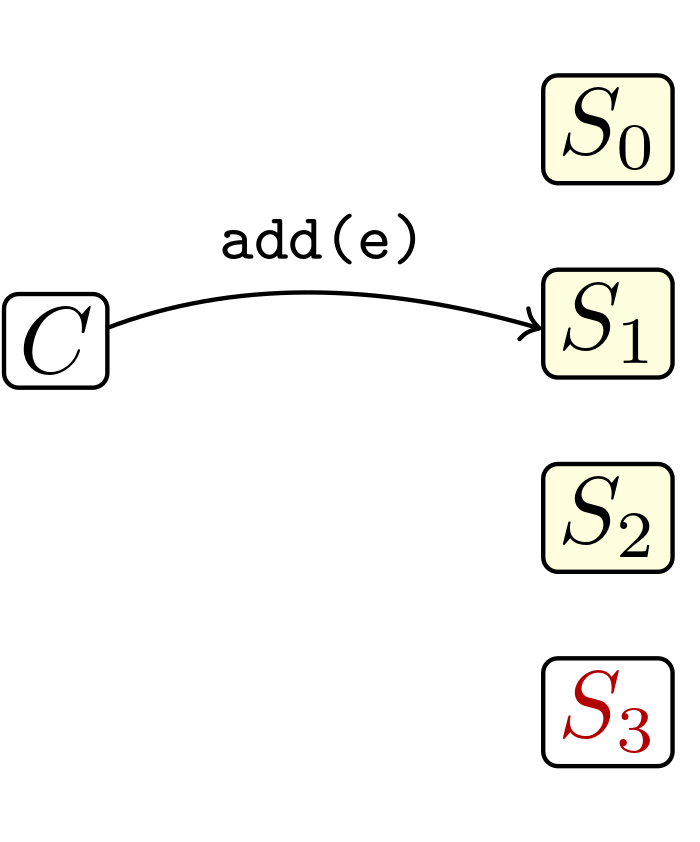
\includegraphics[width = 1.5in]{figures/epoch-proof-0.png}\label{subfig:epoch-proof-a}}
  \hspace{0.5in}
  \subfloat[Época $n$]{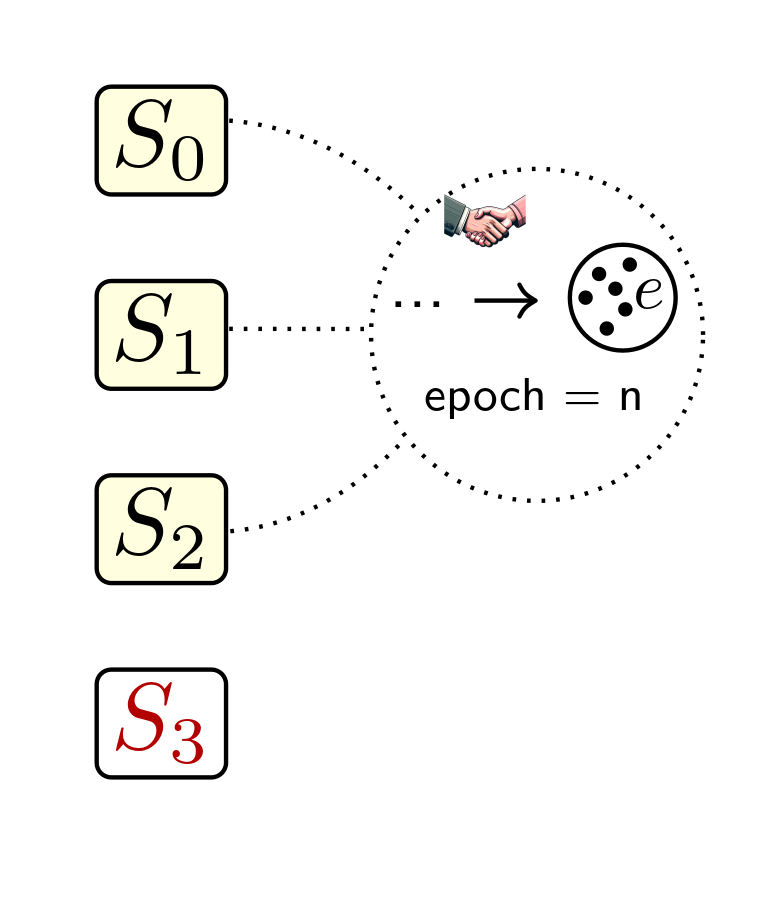
\includegraphics[width = 1.5in]{figures/epoch-proof-1.png}\label{subfig:epoch-proof-b}}\\
  \vspace{0.25in}
  \subfloat[Pruebas de época]{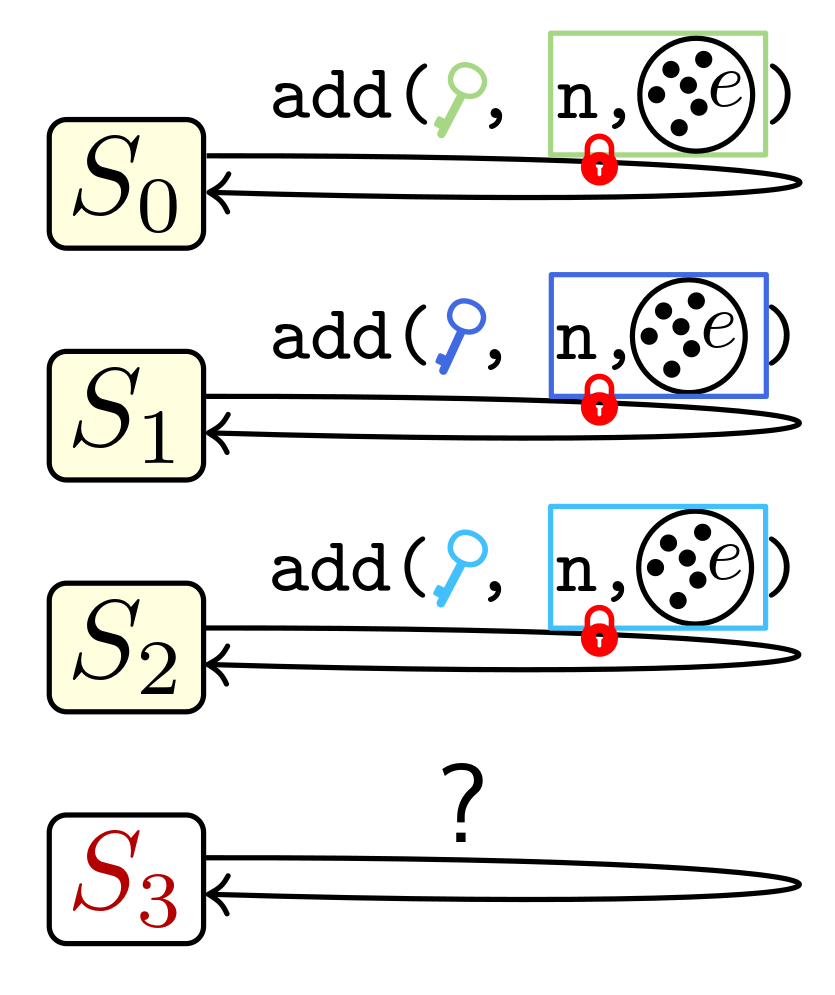
\includegraphics[width = 1.5in]{figures/epoch-proof-2.png}\label{subfig:epoch-proof-c}}
  \hspace{0.5in}
  \subfloat[\<get>]{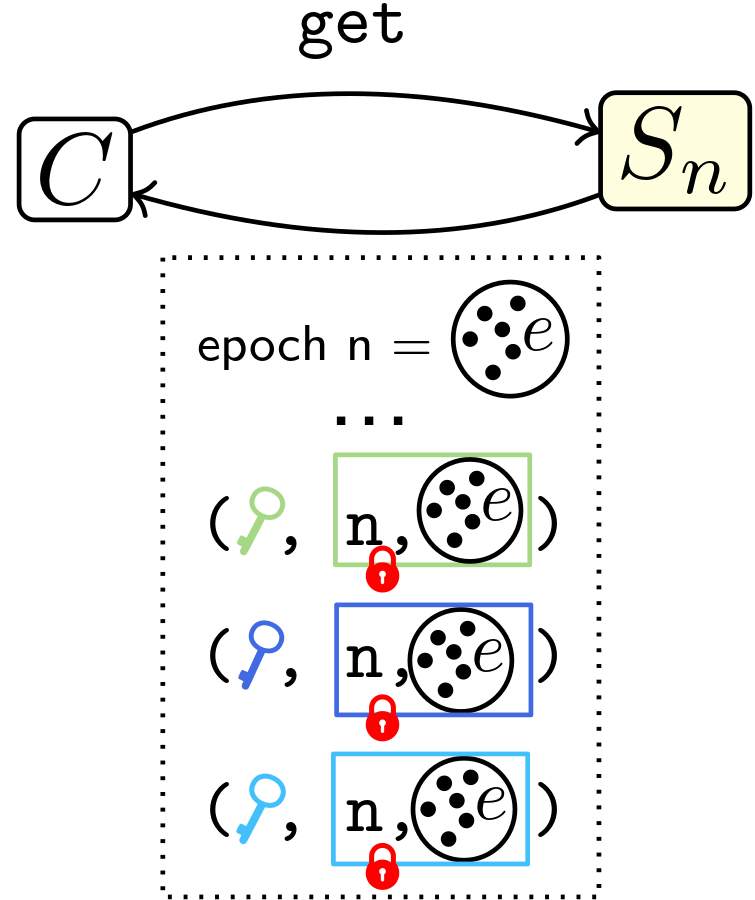
\includegraphics[width = 1.5in]{figures/epoch-proof-3.png}\label{subfig:epoch-proof-d}}
  \caption{Mecanismo de pruebas de época.}
  \label{fig:epoch-proof}
\end{figure}

%
Las claves públicas de los validadores necesitan ser públicamente conocidas para los usuarios.
%
Si un elemento $e$ pertenece a una época que tiene suficientes pruebas, los clientes pueden
concluír que la época es correcta y que $e$ fue éxitosamente insertado en la \setchain.
%
En caso de comunicarse con nodos correctos, solo se requieren una llamada a \<add> y
una llamada a \<get> para estar seguros de que el elemento fue añadido a la \setchain.
%

En la Figura \ref{fig:epoch-proof} se muestra un ejemplo de este mecanismo, en un sistema que cuenta
con un cliente y 4 servidores, de los cuales uno es bizantino (señado en rojo).
%
El cliente invoca $\<add>.(e)$ sobre un servidor cualquiera de la red, sin saber
si es correcto o bizantino, con la intención de agregar un nuevo elemento a la \setchain.
Esto se indica en la Figura \ref{subfig:epoch-proof-a}.
%
Los servidores deciden colaborativamente los elementos pertenecientes a la época $n$.
En la Figura \ref{subfig:epoch-proof-b} se puede ver que $e$ pertenece a dicha época.
%
En la Figura \ref{subfig:epoch-proof-c} se representa que todos los servidores correctos
inyectan un elemento de prueba de época que contiene: el número de época,
la clave pública perteneciente a cada nodo (señalizada con una llave),
y la firma del hash de los elementos de la época $n$ (señalizada con un candado).
%
Luego de esperar cierto tiempo, el cliente invoca \<get> en un servidor cualquiera y,
si obtiene suficientes pruebas de época (en este caso, 3) para la época $n$, entonces
puede estar seguro que el elemento $e$ fue efectivamente agregado a la \setchain.


Las épocas ahora contienen dos tipos de elementos: elementos regulares enviados por
un cliente y elementos de prueba de época; significando que cada elemento de prueba de época
pertenece a su vez a una época. Sin embargo, los elementos de prueba de época no necesitan ser
incluidos como elementos en el hash firmado que es parte de la prueba de época para una época
dada.
%
Consecuentemente, es necesario diferenciar entre elementos regulares y elementos de prueba de época.
%
La validez de los elementos regulares se chequea a través de la ya mencionada función
\<isValidElement>.
%
Sin embargo, un elemento de prueba de época necesita ser validado verificando la firma.
%


\subsubsection{Detalles de implementación}
%Estas pruebas de época pueden implementarse utilizando \textit{Ed25519}~\cite{ed25519}
%como sistema de firmas.

El aspecto criptográfico de la implementación de los elementos de prueba de época se
hace a través del paquete \textit{crypto} de \textit{go-ethereum}, la implementación
del protocolo Ethereum en Golang~\footnote{Disponible en \url{https://pkg.go.dev/github.com/ethereum/go-ethereum/crypto}.}.
%
Este paquete trabaja con el algoritmo de firma digital ECDSA, uno de los esquemas de firmas más
utilizado~\cite{real.world.crypto}.
%
Provee una función \texttt{Sign} que cacula una firma ECDSA.
%
La firma producida se encuentra en el formato $[R || S || V]$, donde $(R, S)$ son los componentes usuales
de una firma ECDSA, y $V$ es 0 o 1.
%
El valor de $V$ es usualmente llamado \textit{bit de recuperación} y permite recuperar inequívocamente,
a partir de la firma y de un hash del mensaje firmado, la clave pública de quien realizó la firma.
%
Sin ese bit de recuperación, el proceso de recuperación de clave pública puede retornar potencialmente
más de un candidato, motivo por el cual se añade dicho bit.
% 
Esta propiedad de recuperación de la clave pública que provee ECDSA es muy útil en contextos con limitaciones
de ancho de banda, en donde la transmisión de la clave pública sería muy costosa.

% This is also useful in bandwidth constrained environments, when transmission of public keys cannot
% be afforded. Entity U could send a signature to entity V , who recovers QU . Entity V can look
% up the public key in some certificate or directory, and if it matches then the signature can be
% accepted. Alternatively, entity U may transmit the signature together with the certificate except
% that the public key is omitted from the certificate. For example, in long certificate chains signed
% with ECDSA, bandwidth can be saved by omission of the public keys.
% Potentially, several candidate public keys can be recovered from a signature. At a small cost, the
% signer can generate the ECDSA signature in such a way that only one of the candidate public keys
% is viable, and such that the verifier has a very small additional cost of determining which is the
% correct public key.

La función \texttt{Ecrecover} es la función de recuperación de clave pública que facilita el paquete \textit{go-ethereum}.
%, la cual dado un hash y una firma, retorna la clave pública
%(en formato descomprimido) que creó dicha firma.
%
Los elementos de prueba de época contienen el número de
época y la firma en el formato mencionado anteriormente, y los clientes pueden, mediante la propiedad de recuperación,
usar la función \texttt{Ecrecover} para
verificar que la firma dada fue, de hecho, generada por un validador conocido.
%

% Chequear si esto es siempre así:
%Este mecanismo de membrecías de elementos a épocas está implementado en la definición de
%\<EndBlock>.

\subsection{Algoritmos}

En esta sección se presentan los algoritmos (en pseudocódigo) necesarios para concluir
la implementación de la versión \vanilla.
%

% Vanilla API - alg0
\begin{figure}[t!]
  \begin{adjustbox}{minipage=[t]{\columnwidth}}
    \begin{algorithm}[H]
      \renewcommand{\thealgorithm}{API Vanilla}         
      \caption{}%
      \label{alg:api-vanilla}%
      \small
      \begin{algorithmic}[1]
            \Function{\<add>}{$transaction$}\label{alg:van_add}
                \State \textbf{return} \<broadcastTx>($transaction$)
                % \Comment {Hit broadcast\_tx\_async RPC endpoint}.
            \EndFunction
      
            \Function{\<get>}{\null}\label{alg:van_get}
                	\State \textbf{return} \<abciquery>()
            \EndFunction
            
        \end{algorithmic}
      \end{algorithm}
	\end{adjustbox}
  \end{figure}

En el Algoritmo~\ref{alg:api-vanilla} se muestra la solución más sencilla a la API
de \setchain.
%
Los clientes agregan elementos invocando indirectamente a
\texttt{Tendermint.Broadcast}, mientras que pueden consultar el estado actual de
la \setchain invocando también de forma indirecta a \texttt{Tendermint.Query}.
%

Para dar una implementación completa de \setchain utilizando Tendermint, además se
deben dar las definiciones de los métodos pertenecientes a la interfaz ABCI
(ver sección~\ref{subsec:abci}). 
%
El Algoritmo~\ref{alg:abci-vanilla} muestra la definición de la ABCI para la versión
\vanilla.
%
Solo se muestran las definiciones de \CheckTx, \DeliverTx, \EndBlock y \Query;
el resto tiene implementaciones triviales.

% Vanilla ABCI - alg1
\begin{figure}[t!]
  \begin{adjustbox}{minipage=[t]{\columnwidth}}
    \begin{algorithm}[H]
      \renewcommand{\thealgorithm}{ABCI Vanilla}         
      \caption{}%
      \label{alg:abci-vanilla}%
      \small
      \begin{algorithmic}[1]
            \State \textbf{Init:} \texttt{epoch} $\leftarrow$ \textbf{-1}, \texttt{next\_epoch} $\leftarrow$ \textbf{0}, \texttt{history} $\leftarrow$ \{\}, \texttt{the\_set} $\leftarrow$ \{\}

            \Function{\<CheckTx>}{$transaction$}\label{alg:van_check_tx}
                \State \textbf{return} \Call{\<isValidTransaction>}{$transaction$}
            \EndFunction
      
            \Function{\<DeliverTx>}{$transaction$}\label{alg:van_deliver_tx}
                \State \<element> $\leftarrow$ \Call{\<getElementFromTransaction>}{$transaction$}
                \If {\Call{\<isValidTransaction>}{$transaction$} and not \texttt{element} in \texttt{history}}
                    \State \texttt{the\_set} \(<- \, \texttt{the\_set} \cup \{\<element>\}\) \label{lst:line:blah2} \label{line:abci-vanilla-set}
                		\State  \texttt{history[next\_epoch]} \(<- \, \texttt{history}[\texttt{next\_epoch}] \cup \{\<element>\}\) \label{line:abci-vanilla-history}
                	\EndIf
                	\State \textbf{return}
            \EndFunction
            
            \Function{\<EndBlock>}{\null}\label{alg:van_end_block}
            		\State \texttt{hash} $\leftarrow$ \<Hash>(\texttt{history[next\_epoch]}, \texttt{next\_epoch})
            		\Comment{Calcular el hash de la época.}
                \State \texttt{epochProof} $\leftarrow$  \texttt{Sign(\texttt{hash}, PRIVATE\_KEY})
                \State \Call{\<add>}{\texttt{epochProof}}
                \State \(\<epoch>  <- \, \texttt{next\_epoch}\)
                \State \texttt{next\_epoch} \( \, <- \texttt{next\_epoch} + 1\)
                \Comment{Cada bloque de Tendermint define una época.}
                \State \textbf{return}
            \EndFunction
            
             \Function{\<Query>}{\null}\label{alg:van_query}
                \State \textbf{return} (\texttt{the\_set}, \texttt{history} up to \texttt{epoch}, \texttt{epoch})            
             \EndFunction
            
            \Function{\<isValidTransaction>}{$transaction$}\label{alg:van_is_valid_tx}
                \State \<element> $\leftarrow$ \Call{\<getElementFromTransaction>}{$transaction$}
                \State \textbf{return} \<isValidElement>(\<element>)
            \EndFunction
            
            \Function{\<getElementFromTransaction>}{$transaction$}\label{alg:van_get_element}
                \State \textbf{return} $transaction$
            \EndFunction
        \end{algorithmic}
      \end{algorithm}
	\end{adjustbox}
  \end{figure}


Chequear si una transacción es válida consiste simplemente en chequear
la validez del elemento, dado que las transacciones contienen un único elemento.
%
Puede parecer absurdo definir la función \texttt{getElementFromTransaction()}
en este caso, debido a que es la función identidad. Sin embargo, la decisión de dar
la definición explícita se basa en enfatizar la diferencia conceptual entre una
transacción de Tendermint y los elementos a añadir en la \setchain.
%

El Tendermint Core envía peticiones \DeliverTx asíncronamente pero en orden
una vez por cada transacción en el bloque.
%
Cuando \DeliverTx se ejecuta, las transacciones ya fueron ordenadas en el consenso global por el protocolo
de Tendermint.
%
Para este algoritmo, la única acción a realizar por parte de la ABCI cuando se recibe una
transacción es añadir el elemento subyacente a la \setchain siempre y cuando el mismo
sea válido.
%
Siempre es necesario chequear del lado de la ABCI si una transacción es válida,
%
%Es importante reparar en que un nodo correcto podría chequear la transacción antes de agregarla a la
%mempool,
%y que el resultado de esa validación cambie para el momento en que ésta arriba a la
%ABCI.
%
ya que un nodo bizantino podría añadir transacciones sin chequear
su validez previamente.
%

Tendermint envía peticiones \EndBlock una única vez por bloque, luego de haber
enviado todas las transacciones dentro del mismo.
%
En este algoritmo, la finalización de un bloque desencadena un incremento de época
y, por lo tanto, cada bloque de Tendermint define una época distitna en la \setchain,
la cual contiene como elementos a las transacciones de dicho bloque.
%
La finalización de un bloque también origina la creación de un elemento de prueba de época
y la posterior invocación a \<add> para añadirlo a la \setchain.

Finalmente, cuando los clientes invocan \<get>, indirectamente inician una llamada
a \<abciquery>, que retorna los valores de $\THESET $, $\HISTORY $ y $\EPOCH $, de acuerdo
a la definición de \setchain.
%
En este caso, $\THESET $ contendrá
todos los elementos para los cuales se hizo \DeliverTx.
Esto incluye elementos desde la época 0 hasta la época que se está construyendo actualmente
(indicada por la variable \texttt{next\_epoch}).
Nótese que los elementos pertenecientes a dicha época pueden estar siendo agregados
a la variable \texttt{history} en 
el momento en que \Query se invoca, por lo que el valor de \texttt{history[\texttt{next\_epoch}]}
podría ser una visión parcial.
Es por esto que se retorna $\HISTORY $ up to $\EPOCH$ y no directamente el valor de la variable
$\HISTORY $.
De otro modo, podría no cumplirse la propiedad \textit{Consistent Gets}
presentada en la sección ~\ref{subsubsec:setchain-properties}.
La variable $\EPOCH$ retornada indica el máximo número de época que fue agregado de
manera completa en $\HISTORY $.
%Es por esto que no sería correcto que $\HISTORY $ incluya elementos
%pertenecientes a la época actual, puesto que podría no cumplir la propiedad \textit{Consistent Gets}
%presentada en~\ref{subsubsec:setchain-properties}.

%$\HISTORY = history up to epoch - 1$, y $\EPOCH = epoch$
%[COMPLETAR. EXPLICITAR QUÉ PINTA TIENE ESTO.]
\subsection{Conclusión}
Si bien los algoritmos descriptos en esta sección implementan \setchain, no se está explotando su idea
principal: relajar el orden total entre los elementos.
%
Aunque diversos elementos pueden pertenecer a una misma época, significando que no hay orden total
entre ellos, por detrás, el protocolo de consenso de Tendermint sí está decidiendo un orden total
entre elementos.
%
% and take advantage of the
% performance improvements that implies.
%

% that then is broken
% when adding the elements from the same block to a specific epoch.


\section{Segunda implementación: Compresschain}\label{sec:compresschain}

Para acercanos al objetivo de \setchain, en esta sección proponemos
%empaquetar elementos en un lote y comprimir dicho lote
%previamente a su difusión.
%
%Se propone
una implementación nueva, llamada \compresschain, que explora
la relajación de orden propuesta por \setchain, aún ejecutando el algoritmo de
consenso de Tendermint por detrás.
%

En lugar de difundir inmediatamente cada elemento añadido por un cliente como una
transacción de Tendermint, una nueva pieza intermedia de software llamada \collector
es responsable de recolectar elementos hasta llegar a un lote lo suficientemente grande,
que es difundido como una única transacción.
%
Esta transacción está formada por los elementos
enviados (potencialmente) por diferentes clientes, convenientemente codificados.
%
El lote de elementos se comprime antes de inyectarse en la red de Tendermint, de ahí el nombre
\compresschain.
%
Una transacción es, entonces, un lote de elementos comprimido.

En este caso, cada una de las transacciones en un bloque de Tendermint define una
nueva época de la \setchain, la cual contiene todos los elementos pertenecientes al lote
comprimido.
Por lo tanto, un mismo bloque de Tendermint involucrará diferentes épocas en la \setchain
(una por cada transacción dentro del bloque).

\subsection{Flujo de mensajes}
Al igual que como se hizo para la versión \vanilla, se presentará el flujo de mensajes usual
que se inicia cuando un cliente invoca \<add>(e).
En la Figura~\ref{fig:compresschain-flow} se muestran los distintos pasos de
este flujo en el contexto de \compresschain.
%

El sistema comienza en su estado inicial.
Como se muestra en la Figura ~\ref{subfig:compress-flow-a}, detrás de la API de \setchain
se encuentra la nueva pieza intermedia \collector.

%

El primer paso se da cuando el cliente envía un elemento $e$, mediante la invocación a \<add>(e), como se
ilustra en la Figura ~\ref{subfig:compress-flow-b}.
Desde el punto de vista del cliente, no hay diferencias en relación a la versión \vanilla, ya que
la existencia del \collector es transparente para él.

%

En la Figura ~\ref{subfig:compress-flow-c} se muestra que el \collector recolecta elementos que envían los distintos clientes y los agrupa
en un lote.
Un lote contiene potencialmente varios elementos enviados por uno o más clientes a un mismo nodo servidor
que corre el Tendermint Core, la aplicación y el \collector.
Cuando el lote se encuentra listo, el \collector tiene una nueva transacción para inyectar en la red de Tendermint.
Esta transacción se presenta en las figuras con un \textit{símbolo de carpeta} gris.

%

Una vez que el lote fue comprimido, el flujo es el mismo que el explicado en la sección anterior para \vanilla: la transacción
que representa al elemento $e$ (y a otros) se chequea contra \CheckTx para determinar si debe ser insertada
en la mempool o descartada.
%
Si llega a la mempool, se espera que luego de un tiempo sea añadida a un bloque de Tendermint y que, eventualmente,
mediante el algoritmo de consenso, este bloque se considere \textit{commited by the network}.
%
Una vez que el bloque fue decidido en el consenso, entonces el Tendermint Core enviará
la secuencia correspondiente de pedidos a la aplicación.
%
Una de las peticiones será \DeliverTx, entregando la transacción correspondiente al lote que contiene a $e$.
%
Esto se observa en las Figuras ~\ref{subfig:compress-flow-d}. ~\ref{subfig:compress-flow-e} y ~\ref{subfig:compress-flow-f}.

%
En el último paso de este flujo se agregan las nuevas épocas a la \setchain.
En contraposición con lo visto en \vanilla, acá se agrega una nueva época por cada transacción (cada petición \DeliverTx).
Las épocas contienen potencialmente más de un elemento porque, de hecho, las transacciones en este contexto representan a más de un elemento
envíado por los clientes.
Estas transacciones sí tienen orden entre ellas, por lo que el número de época asociada a cada una está determinado por el mismo.
En la Figura ~\ref{subfig:compress-flow-g} se muestra que la época $n$ se agregó a la \setchain y uno de sus elementos es $e$. Esta es, justamente, la época asociada
a la transacción que contiene al elemento $e$.


\begin{figure}
  \subfloat[Estado inicial]{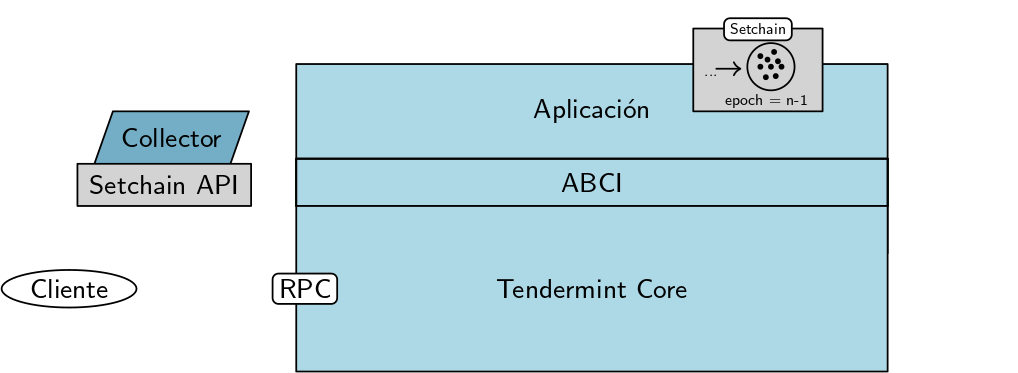
\includegraphics[width = 3.5in]{figures/compresschain-flow-0.png}\label{subfig:compress-flow-a}}
  \subfloat[El cliente invoca \<add>(e)]{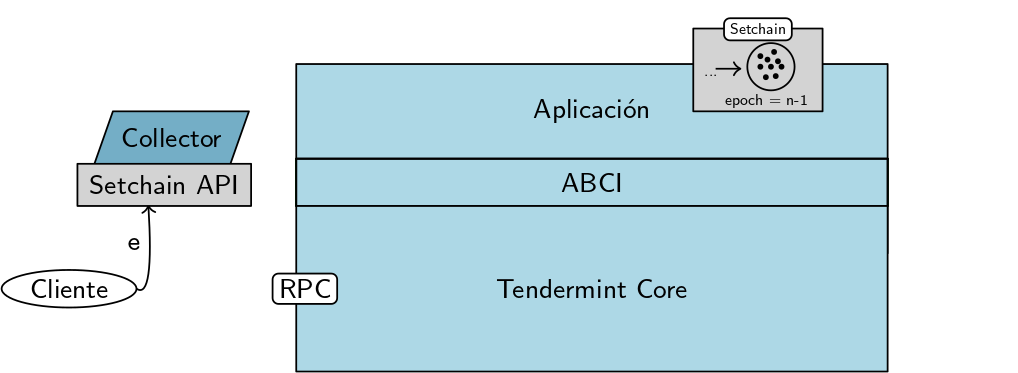
\includegraphics[width = 3.5in]{figures/compresschain-flow-1.png}\label{subfig:compress-flow-b}}\\
  \subfloat[El lote está listo y es difundido]{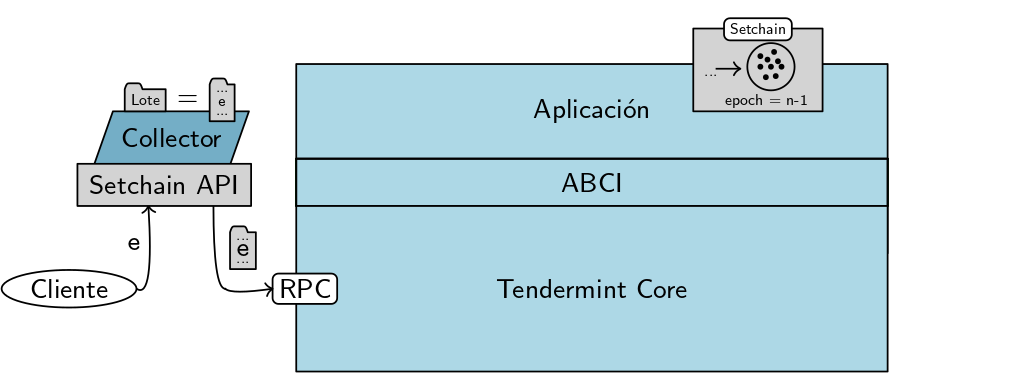
\includegraphics[width = 3.5in]{figures/compresschain-flow-2.png}\label{subfig:compress-flow-c}}
  \subfloat[El lote se chequea contra \CheckTx]{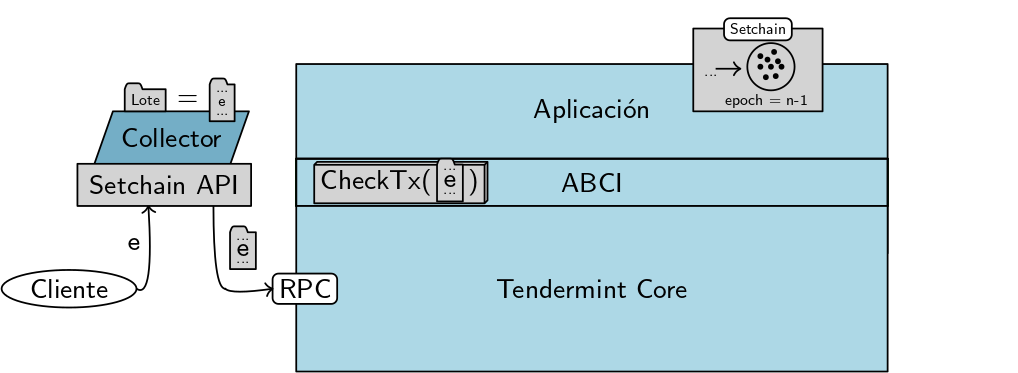
\includegraphics[width = 3.5in]{figures/compresschain-flow-3.png}\label{subfig:compress-flow-d}}\\
  \subfloat[Se consensúa el próximo bloque]{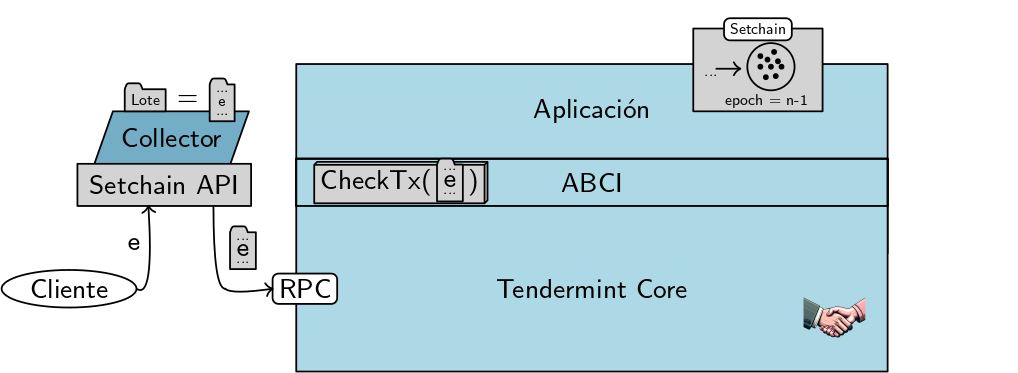
\includegraphics[width = 3.5in]{figures/compresschain-flow-4.png}\label{subfig:compress-flow-e}}
  \subfloat[Se envían los pedidos de la ABCI a la aplicación]{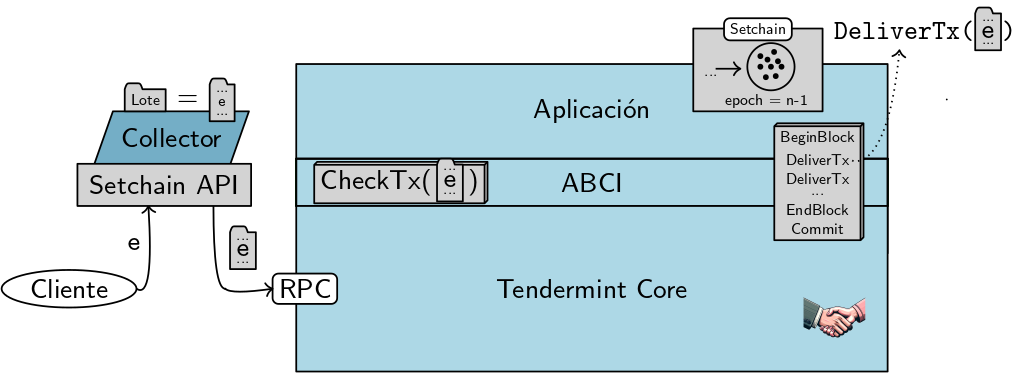
\includegraphics[width = 3.5in]{figures/compresschain-flow-5.png}\label{subfig:compress-flow-f}}\\
  \subfloat[Se agregan las nuevas épocas a la \setchain]{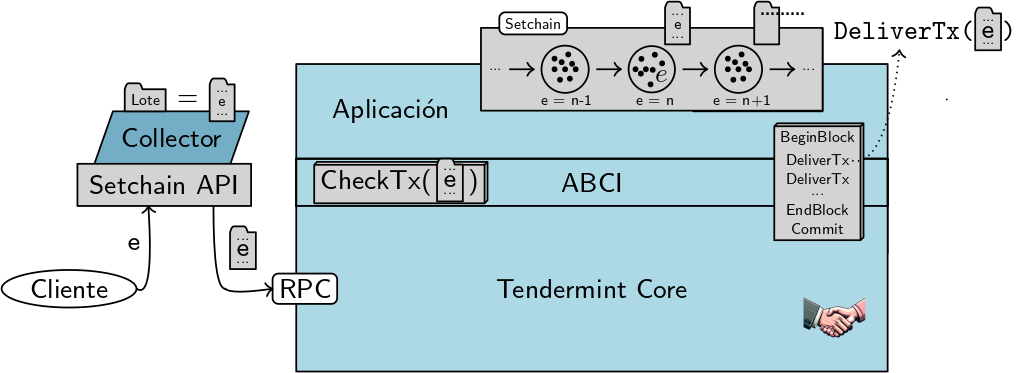
\includegraphics[width = 3.5in]{figures/compresschain-flow-6.png}\label{subfig:compress-flow-g}} 
  \caption{Flujo usual de mensajes para \compresschain}
  \label{fig:compresschain-flow}
\end{figure}

\subsubsection{Detalles de implementación}
La implementación del \collector se hace a través de un servidor HTTP RPC que es accesible para los clientes
mediante la API de \setchain.
%
Para esto se utilizan los paquetes \textit{http} y \textit{rpc}, ambos de la librería estándar de Golang.
%
El paquete \textit{http} proporciona implementaciones para el cliente y el servidor HTTP.
%
El paquete \textit{rpc} provee acceso a los métodos exportados de un objeto (en este caso, el \collector)
a través de una red u otra conexión de entrada/salida.
%
Un servidor registra un objeto, haciéndolo visible como un servicio con el nombre del tipo del objeto.
%
Después del registro, los métodos exportados del objeto (en este caso, únicamente \texttt{AddElement}) son accesibles de forma remota.

%DialHTTP connects to an HTTP RPC server at the specified network address
%// listening on the default HTTP RPC path.

\subsection{Algoritmos}\label{subsec:compresschain-algorithms}
%
% This means that a new
% \setchain API version is defined, which uses the new collector component.
%
% We define a collector in Algorithm.

% To achieve a better throughput in
% terms of size per element broadcasted,  is used.
%

En \compresschain, en lugar de agregar directamente elementos enviados por los usuarios a la red de Tendermint,
primero se recolectan y se comprimen para ser enviados como una única transacción.
Siguiendo la práctica actual de Ethereum, se utiliza el algoritmo
\textit{Recursive Length Prefix} (RLP)~\cite{ethereum} para codificar los elementos individualmente
y el algoritmo de compresión Brotli~\cite{brotli.compressor} para comprimir el lote\footnote{Otros
algoritmos de codificación y de compresión podrían utilizarse de ser necesario.}.

%
Un lote se considera \textit{listo} para ser enviado una vez que, o bien alcanza un tamaño máximo,
o bien una cantidad razonable de tiempo transacurrió desde que el primer elemento llegó. 
%
El Algoritmo~\ref{alg:api-brotli} presenta una nueva definición para la API de \setchain.
En el Algoritmo ~\ref{alg:collector-brotli} se muestra una implementación posible para un
\collector.

% Brotli Collector - alg2
\begin{figure}[t!]
  \begin{adjustbox}{minipage=[t]{\columnwidth}}
    \begin{algorithm}[H]
      \renewcommand{\thealgorithm}{Compress Collector}         
      \caption{}%
      \label{alg:collector-brotli}%
      \small
      \begin{algorithmic}[1]
            \State \textbf{Init:} \texttt{batch} $\leftarrow$ \{\}
      
            \Function{\<AddElement>}{$element$}\label{alg:brotli_add_tx}
            		\If {\<isValidElement>($element$)}
            			\State \texttt{encoded\_element} $\leftarrow$ \texttt{RLP.Encode}($element$)
					        \State \texttt{batch} $\leftarrow$ \texttt{batch} $\cup$ \{\texttt{encoded\_element}\}
                \EndIf
                \State \textbf{return}
            \EndFunction
            
            \smallskip

            \When {\<isReady>(\<batch>)}
              \State \texttt{compressed\_batch} $\leftarrow$  \texttt{Brotli.Compress}(\texttt{batch})
              \State \texttt{Tendermint.Broadcast}(\texttt{compressed\_batch}) \label{line:compresschain-broadcast}
              %\State \Call{\<reset>}{\null}
              \State \texttt{batch} $\leftarrow$ \{\}
            \EndWhen
            
            % \Function{\<reset>}{\null}\label{alg:brotli_reset}
            % 		\State \texttt{batch} $\leftarrow$ \{\}
            %     \State \textbf{return}
            % \EndFunction
        \end{algorithmic}
      \end{algorithm}
	\end{adjustbox}
  \end{figure}



% Compresschain API - 
\begin{figure}[t!]
  \begin{adjustbox}{minipage=[t]{\columnwidth}}
    \begin{algorithm}[H]
      \renewcommand{\thealgorithm}{API Compresschain}         
      \caption{}%
      \label{alg:api-brotli}%
      \small
      \begin{algorithmic}[1]
      
            \Function{\<add>}{$element$}\label{alg:brotli_add}
                \State \textbf{return} \texttt{CompressCollector.AddElement($element$)}
                \Comment {Usar el componente intermedio collector.}
            \EndFunction
      
            \Function{\<get>}{\null}\label{alg:brotli_get}
                	\State \textbf{return} \<abciquery>()
            \EndFunction
            
        \end{algorithmic}
      \end{algorithm}
	\end{adjustbox}
  \end{figure}


%
En \compresschain, un cliente que ejecuta \<add> invoca indirectamente el método \texttt{AddElement}
del \collector.
%
Se realizaron algunas simplificaciones en los algoritmos presentados. Por ejemplo, una condición de carrera
podría ocurrir si varias rutinas agregan elementos a la misma instancia del \collector concurrentemente.
Sin embargo, esto puede resolverse sencillamente gracias al uso de candados.


% After the meeting we decided to call isValidElement() locally in the collector, so the following is not true:
% It is worth mentioning that, as the algorithm shows, the collector adds every element that receives to the batch
% without running any validation on it. While this clearly allows the batch to contain garbage,
% making a \textit{CheckTx()} request to the ABCI app for each new element would mean a decrease in
% performance, as the number of requests would keep constant in the number of elements sent by clients,
% instead of being constant in the number of batches, as it is desired.

%
Para completar nuestra definición, se provee el pseudocódigo para la ABCI de Compresschain en el
Algoritmo~\ref{alg:abci-brotli}.
%
Existen varias diferencias con respecto a la implementación previa de \setchain. Se elaboran
a continuación.
%
% Brotli ABCI - alg1
\begin{figure}[t!]
  \begin{adjustbox}{minipage=[t]{\columnwidth}}
    \begin{algorithm}[H]
      \renewcommand{\thealgorithm}{Compresschain ABCI}         
      \caption{\small }%
      \label{alg:abci-brotli}%
      \small
      \begin{algorithmic}[1]
            \State \textbf{Init:} \texttt{epoch} $\leftarrow$ \textbf{0}, \texttt{history} $\leftarrow$ \{\}

            \Function{\<CheckTx>}{$batch$}\label{alg:brotli_check_tx}
                \State \textbf{return} \Call{\<isValidBatch>}{$batch$}
            \EndFunction
      
            \Function{\<DeliverTx>}{$batch$}\label{alg:brotli_deliver_tx}
				\State \texttt{elements} $\leftarrow$ \Call{\<getElementsFromBatch>}{$batch$}
				\State \Call{\<newEpoch>}{\texttt{elements}}
            		
            		\State \textbf{return}
            \EndFunction
            
            \Function{\<isValidBatch>}{$batch$}\label{alg:brotli_is_valid}
            		\State elements $\leftarrow$ \Call{\<getElementsFromBatch>}{$batch$}
            		
            		\Comment{If at least one element in the batch is valid, then the batch is considered valid.}
            		\For{\texttt{e in} $elements$}
                    \If {\<isValidElement>(\texttt{e}) and not \texttt{e} in \texttt{history}}
                    		\State \textbf{return} \texttt{True}
                    \EndIf
                \EndFor
                \State \textbf{return} \texttt{False}
            \EndFunction
            
            \Function{\<getElementsFromBatch>}{$batch$}\label{alg:brotli_get_element}
                \State \texttt{decompressedBatch} $\leftarrow$ \texttt{Brotli.Decompress}($batch$)
                \State \texttt{elements} $\leftarrow$ \texttt{RLP.Decode}(\texttt{decompressedBatch})
                \State \textbf{return} \texttt{elements}
            \EndFunction
            
            \Function{\<newEpoch>}{$elements$}\label{alg:brotli_new_epoch}
            		\For{\texttt{e in} $elements$}
             		\If {\<isValidElement>(\texttt{e}) and not \texttt{e} in \texttt{history}}
                				\State \texttt{history[epoch]}.AddElement(e)
                				\Comment{Only add new valid elements.}
                    	 \EndIf
                	\EndFor
                	
                	\State \texttt{hash} $\leftarrow$ \<Hash>(\texttt{history[epoch]}, \texttt{epoch})
            		\Comment{Hash epoch (elements and number).}
                \State \texttt{epochProof} $\leftarrow$  \<Sign>(\texttt{hash}, privateKey)
                \State \Call{\<add>}{\texttt{epochProof}}
                	
                	\State \texttt{epoch} $\leftarrow$ \texttt{epoch} + 1
                \State \textbf{return}
            \EndFunction
        \end{algorithmic}
      \end{algorithm}
	\end{adjustbox}
  \end{figure}



La diferencia principal con la implementación \vanilla radica en que las transacciones contienen
potencialmente más de un elemento de usuario. Esto se da porque las transacciones en este contexto
son lotes comprimidos de elementos.
%
Más aún, para recuperar elementos dentro de las transacciones se necesita primero descomprimir
el lote y, una vez que se tiene el lote original, debe RLP-decodificarse para así obtener los elementos
originales enviados por los clientes.
%
Aquellos elementos son los que deben ser agregados a la \setchain. La función \texttt{getElementsFromTransaction()}
muestra este comportamiento.

En la definición de Compresschain, las transacciones de Tendermint contienen, en principio, más de un elemento.
% En la definición de Compresschain, las transacciones de Tendermint pueden contener tanto elementos válidos
% como inválidos.
%
Se necesita definir un nuevo criterio para determinar cuándo una transacción (es decir, un lote de elementos
comprimido) se considera válida.
%
La función \<isValidBatch>~(en el Algoritmo~\ref{alg:abci-brotli}) implementa este nuevo criterio, permitiendo
a las transacciones ser consideradas válidas si al menos uno de sus elementos es válido.
%
La elección de este criterio se basa en que, si bien se espera
que un \collector correcto genere lotes de elementos válidos (puesto que chequea la validez de los elementos
antes de agregarlos),
un \collector bizantino podría incoporar elementos inválidos en un lote.
%
En ese caso, la transacción será considerada válida si al menos uno de sus elementos lo es.
% La elección de este criterio está relacionado con el hecho de que alguien enviando elementos inválidos
% a un nodo no debería privar a los elementos válidos enviados al mismo nodo de
% ser añadidos a la \setchain.
%
A pesar de que una transacción válida puede contener algún elemento inválido,
como se ilustra en el método \<DeliverTx>, solo elementos válidos se agregan a la \setchain,
mientras que los inválidos simplemente se descartan.
%

La última diferencia a mencionar con respecto a \vanilla es que en Compresschain los bloques no delimitan épocas.
Por esta razón no se peresenta una definición para el método \<EndBlock>.
En este caso, las épocas se definen como transacciones: cada lote de elementos define una época.

%
El método \<Query> se comporta de la misma forma que en \vanilla.
% %
% definition was given in this case, as the block does not
% delimit the epoch anymore, but the epoch is defined by all the elements
% belonging to the same Tendermint transaction.
% \textit{DeliverTx()} function
% shows the epoch number increase.

% To dicuss: if epochs are defined by batches, then epochs are generated by the same node.
% This is a new setchain property and may be undesirable. 
\subsection{Conclusión}
\compresschain es una alternativa construida enteramente sobre Tendermint, pero que agrega una capa
intermedia entre el cliente y el Tendermint Core.
De forma completamente transparente tanto para el
cliente como para la pila de Tendermint, muchos elementos enviados potencialmente por diferentes partes
(pero a la misma máquina servidor)
son difundidos dentro de la red de Tendermint como una única transacción.
El algoritmo de consenso
decide el orden de estas transacciones, ignorando por completo cuáles y cuántos elementos hay dentro de ellas.
Si bien los elementos del cliente agrupados dentro de un lote naturalmente tienen un orden específico,
este orden no se decide como parte del consenso y por eso se ignora cuando los elementos son agregados
a una nueva época de la \setchain.

%
El uso de un algoritmo de compresión previo a la inyección de una nueva transacción es una apuesta para mejorar
el rendimiento, medido en cantidad de elementos por segundos, que pueden ser añadidos a la \setchain.
Este enfoque trabaja bajo la hipótesis de que hacer consenso sobre elementos agrupados de forma
eficiente interpretados como unidad representa una mejora en comparación con el consenso usual,
hecho sobre elementos individuales.

\section{Tercera implementación: Hashchain}\label{sec:hashchain}
%
Hashchain se alínea con el concepto introducido en Compresschain; sin embargo, usa
funciones hash en lugar de compresión en Brotli.
%
Mientras que el poder de compresión de las funciones hash puede ser enorme, dado que estas funciones
mapean datos de longitud arbitraria a valores de tamaño fijo, los hashes son irreversibles.
%
Esto significa que debe proveerse un método no trivial para recuperar el lote original de elementos.

% Esto capaz debería sacarlo porque no es claro.
La implementación de Hashcain involucra dos aspectos: una blockchain de Tendermint compuesta por hashes
y una estrategia distribuida de inversión de hashes para obtener los lotes originales de elementos.
%
% We shouldn't mention "consolidated hashes" before explaining it:
%Therefore, we now have to maintain an inverse function for the consolidated
%hashes.

A menudo en esta sección nos tomaremos la libertad de utilizar la expresión \textit{elementos en un hash H}
para referirnos a aquellos elementos pertenecientes al lote $B$, tal que $Hash(B) = H$.

En lugar de usar el \collector de Compresschain (ver Algoritmo ~\ref{alg:collector-brotli}),
ahora utilizamos un \hcollector, que construye un lote de elementos para luego hashearlo
antes de introducirlo a la red de Tendermint.
%
Los lotes hasheados son difundidos como transacciones y compartidos a través de toda la red, definiendo cada
uno de ellos una nueva época en la \setchain, de forma
análoga al enfoque empleado para los lotes comprimidos en \compresschain.

\subsection{Flujo de mensajes}

Al igual que se hizo para las versiones \vanilla y \compresschain, el objetivo es presentar el flujo usual
de la vida de un elemento en el contexto de \hashchain.

%

Retomando la Figura ~\ref{fig:compresschain-flow} de la sección anterior, podemos pensar que el flujo de mensajes
debería ser similar. El cliente se comunica con la API de \setchain, mientras que el \hcollector colecciona elementos
hasta que el próximo lote esté listo para ser hasheado y enviado al Tendermint Core.
Una vez allí es sometido a
\<CheckTx> para determinar si debe ser añadido a la mempool o descartado.


En \compresschain, para decidir si una transacción es válida, debe revertirse el proceso hecho a la misma.
Es decir, descomprimir la transacción para
así obtener los elementos de cliente que la componen y analizarlos de forma individual.
Cuando se piensa en la contraparte para \hashchain, una de las primeras preguntas que surge es cómo se determina si una
transacción (un hash) es válida para ser agregada a la mempool, siendo que no es trivial recuperar los
elementos originales teniendo un hash.

%

La misma pregunta surge luego,
cuando después de consensuado el siguiente bloque llegan las peticiones de la ABCI.
%
El evento \<DeliverTx> dará la indicación de agregar una nueva época a la \setchain, para lo cual también
será necesario conocer los elementos originales con los cuales se formó el hash que está siendo entregado.

Por lo tanto, dado que en el escenario propuesto por \hashchain, tanto \<CheckTx> como \<DeliverTx> reciben hashes como transacciones,
el flujo de mensajes implicará resolver el problema de la obtención de elementos originales provenientes del hash.
A este proceso lo llamaremos \textit{inversión de hashes}.


\subsection{Algoritmo distribuido para la inversión de hashes}\label{subsec:hash-inversion}

%Como ya se mencionón, el \textit{hash collector} adopta un concepto similar al \textit{compression collector}
%de Compresschain. Sin embargo, la definición de la ABCI para Hashchain es considerablemente más compleja.
%
% En este escenario, tanto \<CheckTx> como \<DeliverTx> reciben hashes como transacciones.
%
Debido a la naturaleza irreversible de un hash, un nodo participando de la \setchain no puede traducir
inmediatamente hashes para obtener su lote de elementos original.
%
La ausencia del lote original de elementos hace que \<CheckTx> sea incapaz de verificar los elementos
en la transacción y que \<DeliverTx> no pueda añadir elementos a la \setchain.
%
En este punto, nuestro algoritmo distribuido para la inversión de hashes entra en juego.
%

La propuesta que se hace en este trabajo es comunicarse con un nodo de Tendermint que \textit{conoce el hash}, es decir,
conoce los elementos del cual proviene.
%
Inicialmente, el único nodo que conoce un hash es el creador del mismo.
%
Para distribuir la información sobre quiénes conocen los datos de un hash, las transacciones contienen
no solo el hash del lote, sino además una firma criptográfica.
%
Las firmas que acompañan los hashes indican que un validador específico de Tendermint
(quien firma el hash) afirma conocer el hash y, por lo tanto, si es un nodo correcto,
tiene el lote original de elementos.
%
De esta forma, las transacciones se representan con una tupla $(h, s)$, donde $h$ denota
el valor del hash y $s$ representa la firma obtenida al firmar $h$ con la clave privada
del nodo que conoce el hash.
%
Gracias a la firma es posible comunicarse con el nodo que afirma conocer los datos y obtener
el lote original (si el nodo se comporta apropiadamente).
%
El proceso de petición de inversión de hashes se corre de forma asíncrona para evitar potenciales
retrasos.

El \hcollector mismo es quien se encarga de conseguir el lote asociado a un hash.
%
En la Figura ~\ref{fig:hash-inversion-flow} se muestra el flujo de pedidos que se puede dar
en el proceso de inversión.

\begin{figure}
  \centering
  %\subfloat[Estado inicial]{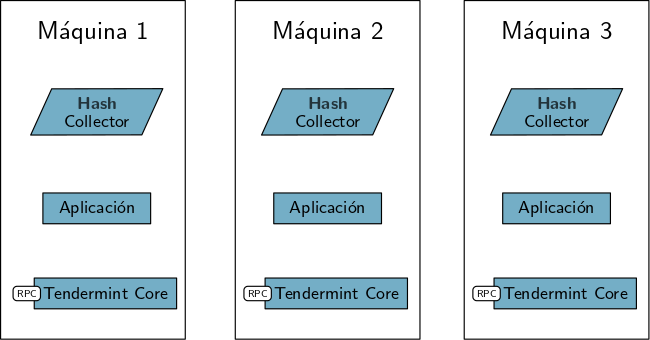
\includegraphics[width = 3.5in]{figures/hash-reversal-0.png}}\\
  \subfloat[La aplicación requiere la inversión de un hash]{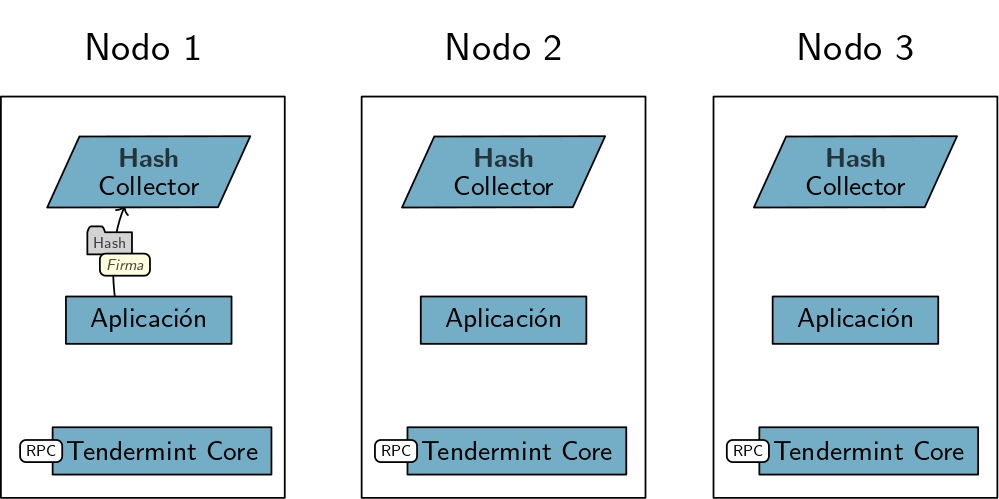
\includegraphics[width = 3.5in]{figures/inversion-hash-1.png}\label{subfig:hash-flow-a}}\\
  \subfloat[El \hcollector conoce el hash]{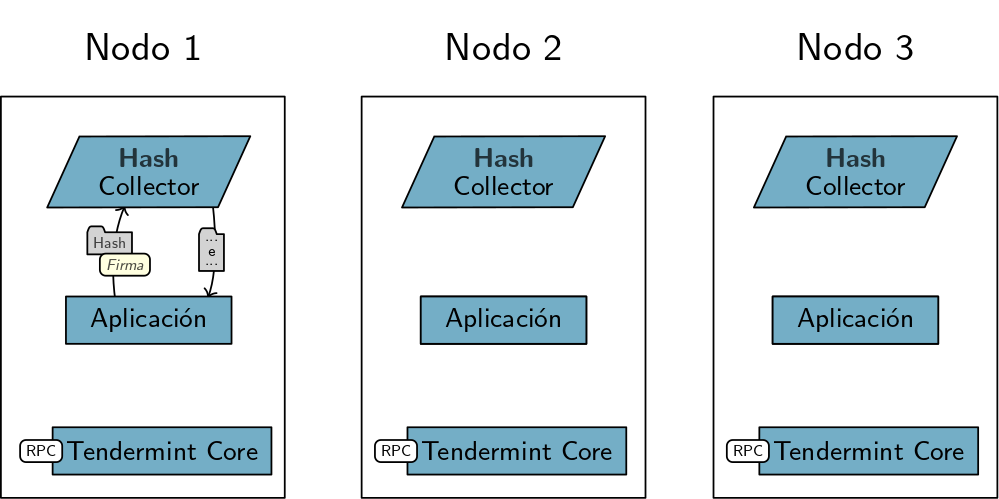
\includegraphics[width = 3.5in]{figures/inversion-hash-2.png}\label{subfig:hash-flow-b}}\\
  \subfloat[El \hcollector no conoce el hash]{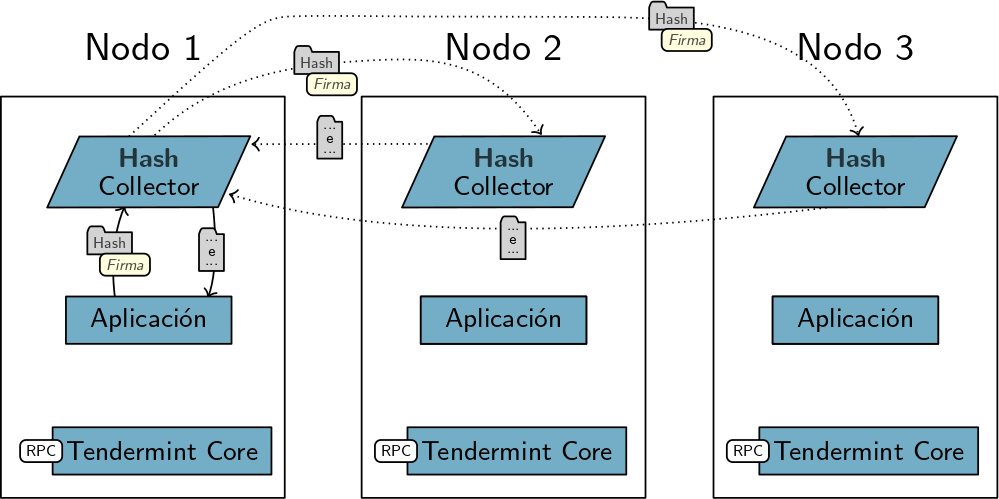
\includegraphics[width = 3.5in]{figures/inversion-hash-3.png}\label{subfig:hash-flow-c}}\\
  \subfloat[Se anuncia a la red el conocimiento de un hash]{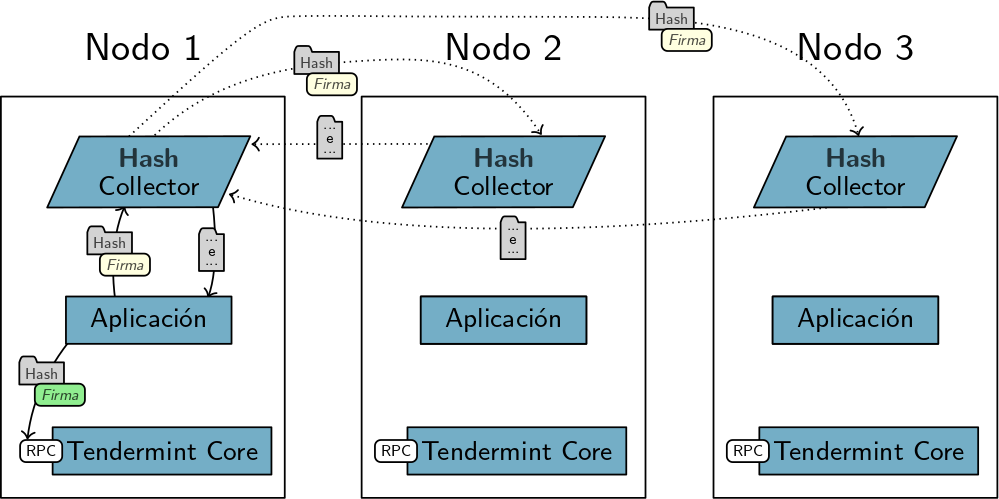
\includegraphics[width = 3.5in]{figures/inversion-hash-4.png}\label{subfig:hash-flow-d}}
  \caption{Flujo usual de mensajes para la inversión de hashes}
  \label{fig:hash-inversion-flow}
\end{figure}

%
En el momento en que la aplicación necesita invertir un hash, se comunica con el \hcollector
para solicitárselo. Esto se observa en la Figura ~\ref{subfig:hash-flow-a}.
%
Si el \hcollector conoce el lote original del hash (por ejemplo, porque fue el \hcollector creador
del mismo), entonces directamente devuelve los elementos asociados a él a la aplicación.
Esto se representa en la Figura ~\ref{subfig:hash-flow-b}.
%

Por el contrario, en la Figura ~\ref{subfig:hash-flow-c} se muestra el caso en que el \hcollector no posee el lote original,
por lo que debe pedírselo al \hcollector correspondiente. Gracias a la firma, es posible determinar
quién es el \hcollector que enuncia tener el lote. Una vez que obtiene el inverso, lo almacena para
futuras peticiones y lo pasa a la aplicación. De esta forma, es transparente para la aplicación
cómo se resuelve el proceso de inversión.

%

En la Figura ~\ref{subfig:hash-flow-d} se muestra el último paso posible de esta comunicación: la aplicación
anuncia a la red sobre el conocimiento de un nuevo hash. Esto ocurre solo cuando la aplicación
efectivamente toma conocimiento de un nuevo hash, ya que anunciar más de una vez que se conoce un
determinado hash generaría tráfico innecesario en la red. Por otro lado, solo se firma el hash si al
menos un elemento en el hash es válido, como se explicará con más detalle en la siguiente sección.
%
En principio, los pares de claves públicas/privadas que sirven para autenticarse
funcionan a nivel nodo: aplicación y \hcollector comparten una misma clave.

\subsubsection{Detalles de implementación}
El \hcollector se implementa, similar a su contraparte en \compresschain, como un servidor HTTP RPC.
%
La comunicación con él por parte del cliente no cambia respecto a lo presentado para el \collector
de \compresschain.
%
La comunicación entre la aplicación y el \hcollector, necesaria para la inversión de hashes,
se hace también de la misma manera.
Es decir, la aplicación actúa como cliente para la comunicación cliente-servidor que establece con
su propio \hcollector.
%
A su vez, es también mediante HTTP RPC que un \hcollector a quien su respectiva aplicación
le solicitó revertir un hash, se comunica con el \hcollector correspondiente, en función de la clave
pública asociada a este (recordar que los hashes a revertir están acompañados de una firma, de la cual
es posible recuperar la clave pública de quien afirma conocer el hash).

La implementación del \hcollector involucra una base de datos persistente capaz de almacenar
las correspondencias entre hashes y lotes.
%
%Cada nueva entrada en esta base de datos es agregada por el \hcollector.
%
A medida que los clientes envían elementos que terminan en la creación de un nuevo hash, o que nuevos hashes se descubren
por medio de otro \hcollector, se agregan nuevas entradas en esta base de datos.
%
Se implementa como una base de datos de tipo clave-valor, utilizando el paquete
\textit{BadgerDB}.
%
Las claves son los hashes y los valores son el lote de elementos asociados.

\subsection{Validación de hashes}

Después de dejar el \hcollector, se espera que los hashes sean chequeados contra \<CheckTx>
para, o bien ser añadidos a la mempool, o bien ser descartados.
%
Para determinar la validez de un hash se necesita chequear los elementos en él. Similar a
\compresschain, los hashes son considerados válidos si al menos un elemento
en el hash es válido.
%
Sin embargo, para un nodo dado, en el punto en que \<CheckTx> corre, no podemos asegurar que el
lote original de elementos sea conocido.

%
Hashchain es optimista en el sentido de que, ante la imposibilidad de correr el chequeo
de las transacciones (debido a la ausencia del lote original), \<CheckTx> considera a los
hashes como transacciones válidas con la esperanza de que sus lotes originales sean enviados
y conocidos más tarde. 

%
La naturaleza optimista de Hashchain tiene consecuencia notables.
%
Como el comportamiento por defecto de  \<CheckTx> es retornar \texttt{True},
se pueden tener transacciones en la blockchain sin conocer los elementos de éstas
(solo conociendo los hashes).
%
Aún más, una transacción puede terminar siendo parte de la blockchain sin que nadie
la haya chequeado previamente, pero pasando el chequeo por el comportamiento optimista.
%
De hecho, este es probablemente el caso para la primera vez que un nuevo hash aparece
en la blockchain, ya que fue consensuado sin que los nodos hayan chequeado realmente los elementos
del lote.
%
%Therefore, we need a way to extract the elements inside the transactions and
%provide the user a uniform view, that of a Setchain.
Por lo tanto, necesitamos definir un criterio para determinar cuándo es seguro
que los elementos en un hash que está en la blockchain sean parte de la \setchain.

% the HashChain living in
% Tendermint, and the \setchain we want to build.
%
Se define un número natural \SPH que establece
el número de firmas que un hash tiene que tener para que los elementos del lote asociado a él
sean considerados elementos a añadir a la \setchain.
%
Estamos únicamente interesados en hashes firmados por al menos \SPH
nodos. A dichos hashes los llamamos \textit{hashes consolidados}.

El número \SPH se define de manera tal que se garantiza que si un hash
consolidó entonces al menos un nodo correcto conoce el lote original del cual proviene.
%
Los elementos de hashes consolidados son los candidatos a pertenecer a la \setchain.
%
Existen casos en los que algunos de dichos elementos pueden no ser añadidos a la \setchain,
por ejemplo, si no son elementos nuevos.
Es decir, si esos elementos ya fueron estampados con un número de época.

%Following the same criteria as in Compresschain, we consider a transaction to
%be valid if we can get the data and validate at least one of its elements.
%
% With this in mind, whenever the ABCI gets the revert of a hash, it runs the
% validation against it, and
%Moreover, if at least one element in the batch is valid, the node verifying the
Cuando un nodo solicita la inversión de un hash, si al menos un elemento en el lote
es válido, el nodo firma el hash con sus propia clave privada y difunde el hash junto
con su propia firma.
%
Al difundir el hash y su firma, el nodo anuncia a la red que conoce el lote detrás de ese hash.
%
De esta forma, los lotes válidos eventualmente consolidarán, significando que sus elementos
serán añadidos a la \setchain.

Para que el algoritmo mencionado funcione, se necesita mantener un registro de cuántas firmas tiene un hash,
así como también un mapeo de hashes a lotes.
%
Durante la ejecución de \<DeliverTx> se chequea la validez de la firma.
%
Si la firma es válida y nueva para el hash en cuestión, se incrementa el contador de
\texttt{firmas por hash}.
%
Además, cada vez que un hash es invertido, se chequea la correctitud del lote original
(es decir, $hash = Hash(originalBatch)$). En caso de éxito, el mapeo de hashes a lotes
es actualizado con el nuevo descubrimiento.

%The first time a hash is passed around, other nodes would see the new hash and
%try to get the data from other servers.
%
%The first one claiming to have the data is the creator of the transaction.


%When a \<get> arrives, we need to get the elements out of the consolidated
%hashes.
% it is necessary to ask for the batch
% corresponding to the hash in the transaction.
%



% Something we discussed with Marga: when the collector creates a hash h and signs it, and broadcast (h, s) every call to CheckTx(h, s) will be true, as no one is expected to have the reverse of h the first time they see it. Because of that, (h, s) in the hashchain doesn't mean that there is at least one good valid element in the h. h could be full of garbage
% A client could contact every collector node with the same elements, and every collector would broadcast (h, sn), with n being the n-collector. This could cause that hash h consolidates, without anyone really having checking elements in h. Is that bad? not too bad, only an empty epoch would occur. Possible fixes: collector hashes elements + pubkey, chain of signatures

\subsection{Consolidación de épocas}\label{subsubsec:consolidation}

En esta implementación las épocas están definidas por todos los elementos en una misma transacción
(es decir, un hash), similar
a lo presentado para \compresschain.
%
En otras palabras, los elementos que provienen del mismo hash consolidado pertenecen a la
misma época.

%
%Now we have to be more careful when adding elements to the setchain, elements
%may appear several times depending on how nodes form batches and
%hashes. \marga{esto no puede pasar tambien en compresschain? un
%  elemento no puede aparecer en varios batches?}
%
% However, what epoch number is that? We need to be more specific
% to define this.

%

Se presentan dos alternativas para asignar un número de época a un hash consolidado.
%
La primera se llama \textit{Consolidación de época actual} (CEC), que significa que 
una vez que un hash consolida, todos sus elementos subyacentes son añadidos a la época actual
(es decir, a la época en la cual la firma número \SPH es vista).
%
La segunda estrategia, \textit{Consolidación de época de primera vista} (FSEC), asigna la época
de acuerdo a cuándo el hash fue visto por privera vez. La asignación de época se lleva
a cabo una vez que el hash consolidó. 
%
Las transacciones
en los bloques de Tendermint están totalmente ordenadas,
por lo tanto ambas estrategias pueden determinar cuál hash ocurrió o consolidó primero, y
todos los nodos correctos estarán de acuerdo en eso.

%
Para ver claramente la diferencia entre estas dos alternativas se presenta un ejemplo.
%
En la Figura~\ref{fig:consolidation_epoch} se ilustran estas dos estrategias para asignar
un número de época a un hash que consolidó cuando \SPH es 3.
%
Como se mencionó en la Sección ~\ref{subsec:hash-inversion}, las transacciones se representan
con una tupla $(h, s)$, donde $h$ es un hash y $s$ es una firma de dicho hash generada con la
clave privada de un validador que afirma conocer los elementos de ese hash.
%
En la figura, el hash $j$ es el primer hash en el bloque $m$, y el hash $k$ es el hash que primero consolida
(es decir, el primero en obtener su tercera firma -denotada como $Firma_{k}2$).
%
Por un lado, la estrategia de consolidación de época actual asigna la época tan pronto como
el hash consolida, estampando los elementos en el hash $k$ con época $a$ primero y luego
a los elementos en el hash $j$ con la época $a+1$.
%
Por el otro lado, la consolidación de época de primera vista no asigna la época al hash $k$
apenas éste consolida, porque el hash $j$ fue visto por primera vez antes que $k$.
%
Dado que el hash $j$ consolida justo después que el hash $k$, los elementos del hash $j$ son
estampados
con la época $a$ y los elementos del hash $k$, con la época $a+1$. 

\begin{figure}
  \centering
  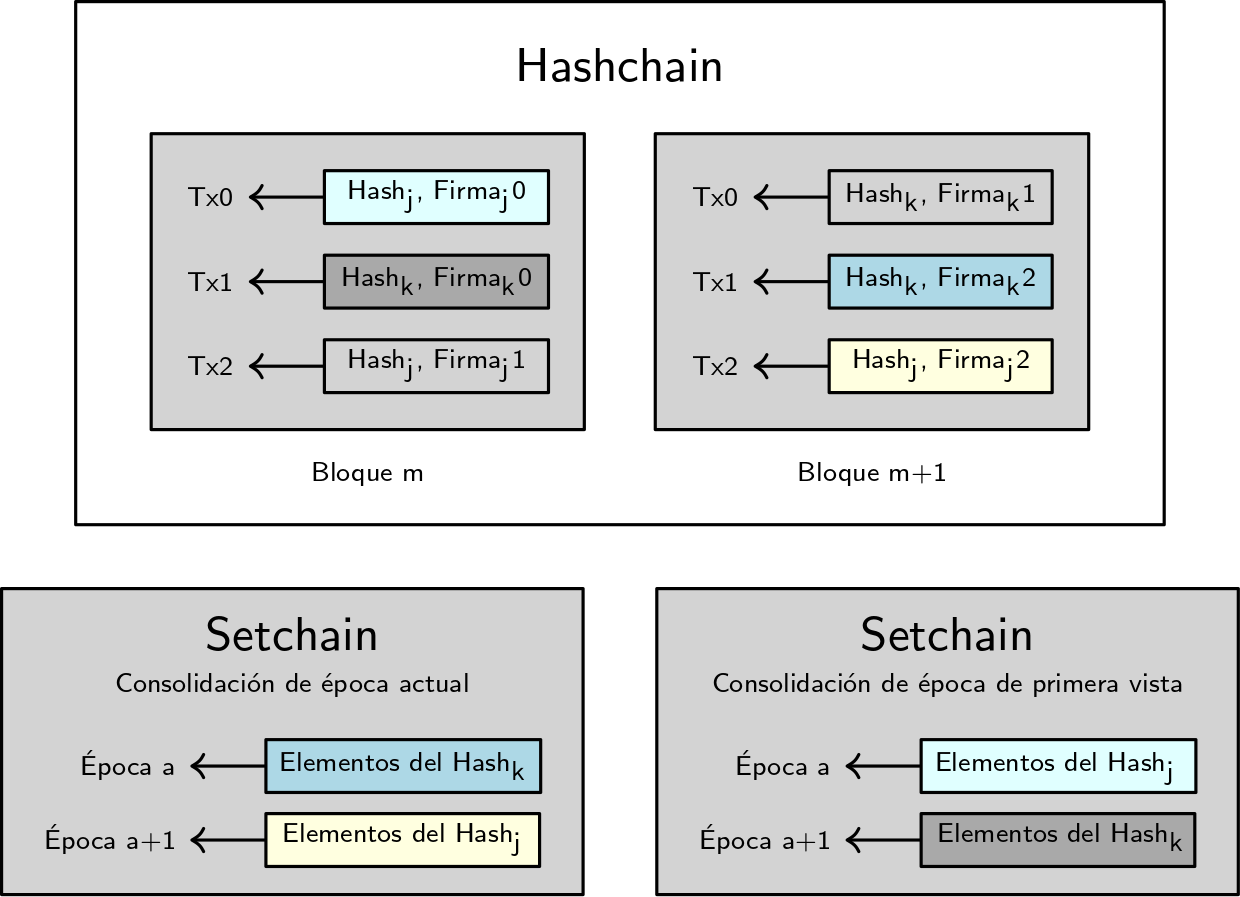
\includegraphics[scale=0.28]{figures/consolidation-example.png}
  \caption{Estrategias de consolidación de épocas}
  \label{fig:consolidation_epoch}
\end{figure}

La variante de consolidación de época de primera vista le otorga a los hashes un período
de gracia en el cual pueden, o bien consolidarse, o bien ser descartados.
%
Dicho período de gracia es necesario; examinemos por qué.
% The grace period is necessary, let
% us briefly examine why.


Suponiendo que no existe período de gracia, si un hash $j$ apareciera por primera vez
antes que el hash $k$, una vez consolidados, los elementos provenientes del hash $j$
serían estampados con la época $E$, mientras que los elementos del hash $k$ serían estampados
con una época $F$ \textgreater \ $E$.
%
Ahora bien, 
%Sea $j$ un hash que fue visto por primera vez en un momento tal que, una vez consolidado,
%se le asignaría la época $E$.
%
si el hash $j$ nunca lograse obtener las \SPH firmas para
consolidar, el hash $k$ (que es \textit{más nuevo} porque fue visto por primera vez
después de $j$) no podría consolidar, dado que sus elementos subyacentes no podrían ser
estampados con una época $F$ \textgreater \ $E$, si la época $E$ no fue definida aún.
%
En la Figura~\ref{fig:grace_period} se muestra un ejemplo de lo mencionado. Los hashes
$k$ y $l$ (e incluso $o$ y $q$) no pueden consolidarse hasta que $j$ consolide o sea rechazada.

\begin{figure}
  \centering
  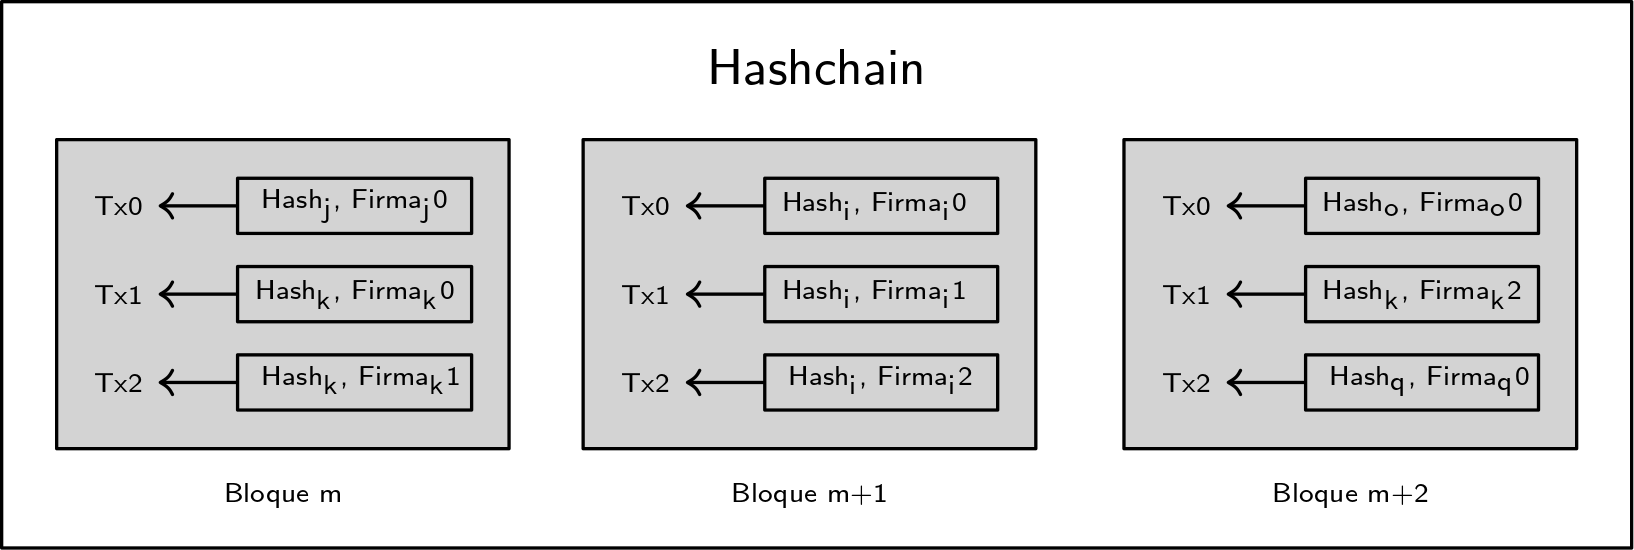
\includegraphics[scale=0.28]{figures/grace-period-example.png}
  \caption{Escenario que requiere período de gracia bajo FSEC.}
  \label{fig:grace_period}
\end{figure}

%
Se concluye entonces que un período de gracia es necesario para garantizar la evolución
exitosa de la \hashchain. 
%
Vale la pena notar que el aspecto crucial en la consolidación de FSEC radica en la ocurrencia
de las \SPH firmas dentro de una ventana equivalente a la duración
del período de gracia.
%
Los hashes que son inicialmente rechazados pueden consolidar en el futuro siempre y cuando
consigan las \SPH firmas dentro del período de gracia.
%
%Los hashes que logran las \SPH firmas terminado el período de gracia
%no consolidarán en la ronda actual; sin embargo, pueden hacerlo en el futuro.

%\subsubsection{Elements Membership Proof}
% Do not use this because we want a proof that specific elements belong to a specific epoch.
%Client processes do not know if they are contacting a Byzantine or correct process. The general idea of a client protocol that wants to ensure that an element is going to be added to the \setchain is to interact with enough servers to guarantee that some are correct. To guarantee contacting at least one correct server, the client needs to send f + 1 messages. However, each element added to the \setchain comes from a consolidated hash. That means that we already have \textbf{SIGNATURES\_PER\_HASH} validator's signatures for that hash. Those signatures may act as a proof for the batch of elements that really belongs to the \setchain. If that proof is added to the epoch as an extra element, a client sending an element, waiting for a while, and then requesting a Get to only one server (hoping it is correct server) may be sure that its element belongs to the \setchain because the epoch comes along a proof of their elements. 

\subsection{Algoritmos}\label{subsubsec:details}

Al igual que se hizo para \vanilla y \compresschain, en esta subsección se presentan los pseudocódigos
para los distintos algoritmos. 

%No definimos un nuevo \texttt{collector} para \hashchain dado que
%es similar al definido
%para \compresschain, con la única diferencia del uso de funciones hash en lugar de funciones de compresión.

En el Algoritmo ~\ref{alg:collector-hash} se muestra una implementación posible para un
\hcollector.
%
La definición de \<AddElement> es similar a la presentada para \compresschain,
con la única diferencia del uso de funciones hash en lugar de funciones de compresión.
%
La definición de \<Reverse> se corresponde con lo explicado mediante la Figura ~\ref{fig:hash-inversion-flow}.
%
Al recibir una petición para la inversión de un hash, si el \hcollector ya conoce el lote asociado al hash
(es decir, lo tiene en su base de datos local), lo retorna.
%
Por el contrario, si no lo conoce, se comunica con el \hcollector correspondiente para obtenerlo.  

% No collector piece for Hashchain appears as it is similar to the already
% presented collector for Brotli, employing hash functions instead of Brotli
% compression.
En el Algoritmo ~\ref{alg:api-hashchain} se define la API de \setchain.

% shows how a new collector is
% used now in order to add elements to the \setchain.

Finalmente, en relación a la definición de la ABCI, se muestra una posible implementación para
\hashchain utilizando la estrategia de consolidación de época actual en el Algoritmo ~\ref{alg:abci-hash1}
y ~\ref{alg:abci-hash2}.

Es importante notar que en el algoritmo el método \<Query> inicia la construcción de \<history>, además de
la difusión de pruebas de época.
%
Aunque este enfoque es empleado por su claridad, un nodo que recibe consultas
no muy frecuentemente podría experimentar retrasos en la generación de pruebas de época.
%
Para evitar esto, el proceso de construcción de \<history> y las pruebas de época podrían ser ejecutadas
periódicamente mediante planificación, independientemente de la petición de consultas.

%
A diferencia de lo visto para \<Query> en \vanilla y \compresschain, en este caso, la diferencia entre $\THESET $ y $\HISTORY $
no radica en las épocas a medio construir, puesto que el proceso de construcción de épocas es atómico.
En este contexto, en $\THESET $ se encuentran todos los elementos que el nodo firma y difunde, aún antes de ser estampados con un
número de época. Notemos que esto es correcto puesto que eventualmente todos los nodos correctos van a recibir el lote correspondiente
y firmarlo, por lo que con seguridad sus elementos tendrán un número de época asignado en el futuro.


% Hash Collector - alg3
\begin{figure}[t!]
  \begin{adjustbox}{minipage=[t]{\columnwidth}}
    \begin{algorithm}[H]
      \renewcommand{\thealgorithm}{Hash Collector}         
      \caption{}%
      \label{alg:collector-hash}%
      \small
      \begin{algorithmic}[1]
            \State \textbf{Init:} \texttt{batch} $\leftarrow$ \{\}
      
            \Function{\<AddElement>}{$element$}\label{alg:hash_add_tx}
            		\If {\<isValidElement>($element$)}
            			\State \texttt{encoded\_element} $\leftarrow$ \texttt{RLP.Encode}($element$)
					        \State \texttt{batch} $\leftarrow$ \texttt{batch} $\cup$ \{\texttt{encoded\_element}\}
                \EndIf
                \State \textbf{return}
            \EndFunction

            \smallskip

            \When {\<isReady>(\<batch>)}
              \State \texttt{hash} $\leftarrow$  \texttt{Hash}(\texttt{batch})
              \State \texttt{Tendermint.Broadcast}(\texttt{hash})
              %\State \Call{\<reset>}{\null}
              \State \texttt{batch} $\leftarrow$ \{\}
            \EndWhen

            \Function{\<Reverse>}{$h$, $s$}\label{alg:hash_request_tx}
              \If {\texttt{DATA\_BASE}.Get($h$) \texttt{is not null}}
                \State \texttt{batch} = \texttt{DATA\_BASE}.Get($h$)
                \Comment{Obtener el lote de la base de datos local.}
              \Else
                \State \texttt{public\_key} = \<RecoverPK>($s$)
                \State \texttt{collector} = \texttt{BuildCollector(public\_key)}
                \State \texttt{batch} = \texttt{collector}.\Call{\<Reverse>}{$h$, $s$}
                \Comment{Obtener el lote mediante otro collector.}
                \State \texttt{DATA\_BASE}.Set($h$, \texttt{batch})
                \Comment{Añadir la nueva entrada a la base de datos local.}
              \EndIf
              \State \textbf{return} \texttt{batch}
            \EndFunction
            
            % \Function{\<reset>}{\null}\label{alg:hash_reset}
            % 		\State \texttt{batch} $\leftarrow$ \{\}
            %     \State \textbf{return}
            % \EndFunction
        \end{algorithmic}
      \end{algorithm}
	\end{adjustbox}
  \end{figure}


% Setchain API - 
\begin{figure}[t!]
  \begin{adjustbox}{minipage=[t]{\columnwidth}}
    \begin{algorithm}[H]
      \renewcommand{\thealgorithm}{API Hashchain}         
      \caption{}%
      \label{alg:api-hashchain}%
      \small
      \begin{algorithmic}[1]
      
            \Function{\<add>}{$element$}\label{alg:hash_add}
                \State \textbf{return} \texttt{HashCollector.AddElement($element$)}
                \Comment {Use the middleware collector component}.
            \EndFunction
      
            \Function{\<get>}{\null}\label{alg:hash_get}
                	\State \textbf{return} \<abciquery>()
            \EndFunction
            
        \end{algorithmic}
      \end{algorithm}
	\end{adjustbox}
  \end{figure}


% Hash ABCI - alg4
\begin{figure}[t!]
  \begin{adjustbox}{minipage=[t]{\columnwidth}}
    \begin{algorithm}[H]
      \renewcommand{\thealgorithm}{ABCI Hashchain - Parte 1}
      \caption{Consolidación de época actual}%
      \label{alg:abci-hash1}%
      \small
      \begin{algorithmic}[1]
            \State \textbf{Init:} \texttt{next\_epoch} $\leftarrow$ \textbf{0}, \texttt{history} $\leftarrow$ \{\}, \texttt{the\_set} $\leftarrow$ \{\}, \texttt{hash\_to\_signatures} $\leftarrow$ \{\}, \texttt{epoch\_to\_hash} $\leftarrow$ \{\}, \texttt{hash\_to\_batch} $\leftarrow$ \{\}

            \Function{\<CheckTx>}{$hash, signature$}\label{alg:hash_check_tx}
				\If {\<isValidSignature>($hash, signature$)}
            			\If {\texttt{hash\_to\_batch}[$hash$] \textbf{exists}}
            				\State \textbf{return} \Call{\<isValidBatch>}{\texttt{hash\_to\_batch}[$hash$]}
            			\EndIf

						\Comment{Si el nodo no tiene el lote original, lanzar una rutina asíncrona que solicita el lote.}
            		
                		\State \textbf{spawns} \Call{\<reverse>}{$hash, signature$}
                		\State \textbf{return True}
						\Comment{En caso de ausencia de información, retornar True.}
                	\Else
                		\State \textbf{return False}
                	\EndIf
            		\EndFunction
      
            \Function{\<DeliverTx>}{$hash, signature$}\label{alg:hash_deliver_tx}
            		\If {\<isValidSignature>($hash, signature$)}
            			\State \texttt{hash\_to\_signatures}[$hash$] $\leftarrow$ \texttt{hash\_to\_signatures}[$hash$] $\cup$  \{$signature$\}
            			\If {\Call{\<shouldConsolidateHash>}{$hash$}}
            				\State \texttt{epoch\_to\_hash[next\_epoch]} $\leftarrow$ $hash$
            				\State \texttt{next\_epoch} $\leftarrow$ \texttt{next\_epoch} + 1
            				\If {not \texttt{hash\_to\_batch}[$hash$] \textbf{exists}}
                				\State \textbf{spawns} \Call{\<reverse>}{$hash, signature$}
                			\EndIf
               	 	\EndIf
               	 \EndIf
                \State \textbf{return}
            \EndFunction
            
            \Function{\<Query>}{\null}
            		\State \texttt{lastEpochInHistory} $\leftarrow$ max(\texttt{history})
            		\For{\texttt{i in (\texttt{lastEpochInHistory, next\_epoch})}}
            			\State \texttt{hash} $\leftarrow$  \texttt{epoch\_to\_hash[i]}
             		\If {\texttt{hash\_to\_batch}[\texttt{hash}] \textbf{exists}}
                			\State elements $\leftarrow$ \Call{\<getElementsFromBatch>}{\texttt{hash\_to\_batch}[\texttt{hash}]}
            				\For{\texttt{e in elements}}
								\Comment{Agregar solo elementos nuevos y válidos.}
             					\If {\<isValidElement>(\texttt{e}) and not \texttt{e} in \texttt{history}}
									\State  \texttt{history[i]} \(<- \, \texttt{history}[\texttt{i}] \cup \{\texttt{e}\}\) \label{line:abci-hashchain-history}
									%\State \texttt{history[i]}.AddElement(e)
                    	 		\EndIf
                    	 	\EndFor
                    	    \State \texttt{epoch\_hash} $\leftarrow$ \<Hash>(\texttt{history[i]}, \texttt{i})
            				%\Comment{Hash epoch (elements and number).}
                			\State \texttt{epoch\_proof} $\leftarrow$  \texttt{Sign(\texttt{epoch\_hash}, PRIVATE\_KEY)}
               			\State \Call{\<add>}{\texttt{epoch\_proof}}
               		 \Else
						\State \texttt{epoch} \(<- \, \texttt{i - 1}\)
						\Comment{Guardar el número de la última época completa.}
               		 	\State \textbf{break}
                    	\EndIf
                	\EndFor
            		\State \textbf{return} (\texttt{the\_set}, \texttt{history}, \texttt{epoch}) 
            	\EndFunction

        \end{algorithmic}
      \end{algorithm}
	\end{adjustbox}
  \end{figure}
  
  \begin{figure}[t!]
  \begin{adjustbox}{minipage=[t]{\columnwidth}}
    \begin{algorithm}[H]
      \renewcommand{\thealgorithm}{ABCI Haschain - Parte 2}         
      \caption{\small Consolidación de época actual}%
      \label{alg:abci-hash2}%
      \small
      \begin{algorithmic}[1]
            	\Function{\<reverse>}{$hash, signature$}\label{alg:hash_revert}
                \State \texttt{original\_batch} $\leftarrow$ \texttt{my\_collector}.\Call{\<Reverse>}{$hash, signature$}
                \If {Hash(\texttt{original\_batch}) = $hash$}
					\State \texttt{hash\_to\_batch}[$hash$]  $\leftarrow$ \texttt{original\_batch} \label{line:abci-hashchain-hash-to-batch}
                		%\If {\Call{\<isValidBatch>}{\texttt{original\_batch}}}
							\For{\texttt{e in \Call{\<getElementsFromBatch>}{original\_batch}}}
								\If {\<isValidElement>(\texttt{e})}
									\State \texttt{the\_set} \(<- \, \texttt{the\_set} \cup \{\texttt{e}\}\) \label{line:abci-hashchain-the-set}
								\EndIf
							\EndFor
                			\State \texttt{my\_signature} $\leftarrow$ \<Sign>($hash$, \texttt{PRIVATE\_KEY})
                			\State \texttt{Tendermint.Broadcast}($hash$, \texttt{my\_signature})
						%\EndIf   
				\EndIf             	
                	\State \textbf{return}
            \EndFunction
            
             \Function{\<shouldConsolidateHash>}{$hash$}\label{alg:hash_consolidated}
            		\State \textbf{return} \textbf{\#}\texttt{hash\_to\_signatures}[$hash$] = \texttt{SIGNATURES\_PER\_HASH}
            \EndFunction

        \end{algorithmic}
      \end{algorithm}
	\end{adjustbox}
  \end{figure}
  


% Make this appears after all the algorithms.

\subsection{FSEC vs CEC}
En esta sección se comparan las estrategias FSEC y CEC a partir de la idea de ataques de \textit{front-running}.
En el contexto de las blockchains, un ataque de front-running~\cite{frontrunning} refiere a una situación en donde
un actor malicioso explota conocimiento sobre transacciones pendientes para obtener una ventaja
desleal. Debido a que las transacciones pendientes son públicas, un usuario malicioso puede
observar las transacciones que le llegan a una víctima, construir una nueva transacción y luego
encontrar una forma de ubicarla antes que la transacción de la víctima. En la red Ethereum, esta
\textquotedblleft forma \textquotedblright de colocar una transacción antes de otra es usualmente
llevada a cabo mediante pagos: o bien pagando impuestos de transacción (\textit{transacction fees}) más altos
que la víctima, o haciendo pagos directos a ciertos validadores.
%

\subsubsection{Front-running en \hashchain}
En esta sección analizaremos qué clase de ataque de front-running puede suceder al nivel de abstracción de \hashchain.
%¿Qué clase de ataque de front-running puede suceder al nivel de abstracción de \hashchain?
Supongamos que un validador $v$ recibe una transacción $(h_k, s_{k}0)$, donde $h_k$ es un hash,
y $s_{k}0$ una firma de aquel hash (la primera que el validador recibe).
Un validador especulador puede firmar él mismo la
transacción y difundirla (el comportamiento esperado), o puede ignorarla (un posible comportamiento
malicioso). Si el validador la firma y la difunde, entonces está colaborando para que el hash
consolide (y, por lo tanto, los elementos provenientes de él se agreguen a la  \setchain).
En caso contrario, no contribuirá a que el hash consolide, potencialmente causando retrasos
en la consolidación.
%

%¿Cuál es la diferencia entre ambas estrategias de consolidación presentadas?
%
Las estrategias de consolidación presentadas en la sección anterior tienen distintos comportamientos.
En la estrategia FSEC, si una transacción no obtiene las \SPH firmas
dentro del período de gracia, el hash no consolidará en aquella ronda (pero podría hacerlo
en el futuro).
%
En la estrategia CEC, el hash no consolidará hasta obtener las \SPH firmas,
sin tener ningún período de gracia para ello.
%
En este punto, las estrategias no parecen tener diferencias fundamentales. Sin embargo, el aspecto
interesante se da en el escenario alternativo: cuando las transacciones finalmente son añadidas a la
\setchain.
%

Supongamos que $v$ ve una transacción $t_0 = (h_k, s_{k}0)$ y quiere ejecutar un ataque de front-running.
Para lograrlo, ignora la transacción, pero difunde su propia transacción firmada $t_1 = (h_l, s_{l}0)$,
esperando que $t_1$ finalmente sea estampada con una época menor que $t_0$.
%

Bajo el comportamiento FSEC, $h_k$ fue visto por primera vez antes, por lo que si logra las
\SPH firmas dentro del período de gracia, consolidará y los elementos
en el hash serán estampados con una época menor a la de $t_1$.
%
Notemos que esto es completamente independiente del número de firmas que $h_l$ logre y la velocidad
a la cual lo haga. El hash $h_l$ podría incluso consolidar (llegar a su firma \SPH)
antes que $h_k$.
%

Por el otro lado, bajo el comportamiento CEC la situación es básicamente una carrera entre $h_k$ y
$h_l$: el primero en obtener las \SPH firmas será el primero en consolidar y,
por lo tanto, sus elementos serán estamapdos con una época más temprana.
%

Como ya se mencionó, 
la estrategia FSEC toma en consideración no solo el momento en el cual los hashes consolidan, sino
también el momento en que las transacciones fueron vistas por primera vez.
%
En principio, esta característica se puede considerar un aspecto valioso en la mitigación de ataques
de front-running, dado que las transacciones observadas primero son probablmente las legítimas y
originales.
%At girst glance, we could think that this property is an interesting point to go against
%front-running attacks, as first-seen transactions are probably the legit original transactions.
Sin embargo, la estrategia FSEC viene con algunos apesctos negativos no triviales que se presentan
a continuación.


Dado que la época en FSEC es determinada por el momento en el cual el hash fue visto por primera vez, 
la estrategia de alguna manera \textit{reserva} el número de época para la transacción específica.
Si $v$ quiere que un hash $h_k$ consolide únicamente si puede hacerlo antes que otro hash
$h_l$ (y no necesita conocer los elementos de $h_l$ desde antes), $v$ podría hacer lo siguiente.
%
Primero, difunde la transacción de modo que todos los validadores reservan el número de época para ella.
%
Luego, $v$ no revierte el hash $h_k$ a nadie, porque quiere esperar hasta que el hash $h_l$ aparezca
y obtenga suficientes firmas.
%
Una vez que esto sucede, y es seguro que el hash $h_l$ consolidará, $v$ comienza a revertir su hash
$h_k$ a todos sus pares, esperando que el hash logre las \SPH firmas dentro del período de gracia.
Si es exitoso, luego $v$ habría cumplido su objetivo: los elementos del hash $h_k$ serían estampados
con una época menor que los elementos provenientes del hash $h_l$.
%

Esta situación es particularmente interesante porque el validador $v$ puede hacer algo
suceder en el pasado (elemento del hash $h_k$ se estampan con época $e$) teniendo información
del futuro (elementos del hash $h_l$ se estampan con época $e+n$). A este ataque en el contexto
de \hashchain lo llamamos \textit{el ataque del clarividente}.
%

En principio, intentar hacer algo similar bajo el esquema CEC no sería posible, dado
que una vez que el hash $h_l$ consolidó, sus elementos son estampados con un número de época menor
a cualquier hash que aún no consolidó.
%

\subsubsection{El ataque del clarividente}

Volvamos a este ataque con un ejemplo. Supongamos que hay un juego de apuestas simple en donde
las apuestas y el resultado final se publican en la \hashchain. El juego es sencillo: los usuarios
pueden votar por A o por B. Se sabe que el resultado ganador (A o B) se publica en determinado momento,
y todo aquel que haya votado por el resultado ganador recibirá el premio.
%

Si $v$ es un validador que quiere ganar este juego haciendo trampa, podría votar tanto por A
como por B justo antes del momento en el que se sabe que la compañía publicará el resultado ganador.
%
Dado que $v$ difundió dos transacciones (una votando por A y otra votando por B) antes de que la
transacción con el resultado ganador aparezca, todos los validadores reserverán un número de época
anterior al del resultado. Después de esto, $v$ no revertirá el hash asociado con estas transacciones
hasta que esté seguro de cuál es el resultado ganador (que efectivamente será añadido a la \hashchain).
%
Una vez que se asegura el resultado ganador, solo dará a conocer la inversa del hash que contiene la apuesta
por el resultado ganador. Si obtiene las firmas necesarias durante el período de gracia,
sus transacciones serían estampadas con un número de época anterior que la transacción de los resultados,
y por lo tanto, $v$ ganaría el juego haciendo trampa.

\subsection{Conclusión}

\hashchain emplea la estrategia introducida en \compresschain mediante el uso del \collector,
agregando una capa
intermedia entre el cliente y el Tendermint Core.
Trabaja también sobre la misma hipótesis: hacer consenso sobre elementos agrupados de forma eficiente
interpretados como unidad representa una mejora en comparación con el consenso usual, hecho sobre elementos
individuales.

La novedad en \hashchain es que, en lugar de usar un algoritmo de compresión, utiliza funciones hash
para reducir la sobrecarga de la red.
De esta forma se profundiza la idea original presentada en \compresschain, ya que una función hash
puede ser vista como un método de compresión con un ratio potencialmente muy alto (dado que convierte
texto plano de longitud arbitraria en un hash de longitud fija).

Aunque reduzca el tráfico de la red (haciendo consenso sobre transacciones pequeñas
y de tamaño fijo), el uso de funciones hash requiere una forma de
invertirlos para así obtener los elementos originales.
Para resovler esto, se diseñó
un algoritmo distribuido, tolerante a fallas bizantinas, que trabaja como un objeto
distribuido de resolución de hashes.


% While reducing network traffic, the use of hash functions requires a way to
% get the elements back. To solve this, we designed a new distributed Byzantine-
% tolerant algorithm working as a hash-resolution distributed object.

%Considerando esto, tendríamos una implementación de \setchain de mundo real.
%Dado que los nodos no conocen de ante mano los elementos en un
%hash, el consenso consiste en elegir cuál época será la siguiente.
% Putting both
% solutions together, we would have a real-world Setchain implementation.
% Hashchain is the closest solution to Setchain without using a set-consensus
% algorithm. Since nodes do not know a priory the elements inside a hashed set,
% consensus then consists in choosing what epoch is going to go next.
% Sin embargo, puesto que Tendermint tiene una mempool y una red de difusión (\textit{gossip network}),
% los elementos se difunden, y los hashes tienen el conjunto más grande de elementos conocidos
% por el nodo que propone la próxima época.

% However,
% since in Tendermint we have a mempool and a gossip network, elements are
% gossiped around, and hashes have the biggest set of elements known to the node
% proposing the next epoch.
% Our results are exciting but inconclusive. On the one hand, we presented three
% algorithms ready to be deployed implementing Setchain specification. While on
% the other hand, we have not yet tested and experimented on the most interesting
% one: Hashchain. Leaving the implementation of Hashchain as future work. Fi-
% nally, we also want to run intense tests on each of the implementations employing
% Tendermint deployment systems.
%%% Local Variables:
%%% TeX-master: "article.tex"
%%% TeX-PDF-mode: t
%%% End:
